% License: LaTeX Project Public License 1.3c
% file JCMS_revised_v2.tex 
% Revised manuscript for Journal of Creative Music Systems

\documentclass[a4paper]{article}

\usepackage{JCMS}           % load package
\usepackage[utf8]{inputenc} % allow utf-8 input
\usepackage[T1]{fontenc}    % use 8-bit T1 fonts
\usepackage{type1cm}        %
\usepackage{booktabs}       % professional quality tables
\usepackage{multirow}       % tables with multi-row cells
\usepackage{amsmath}        % math environments (align, etc.)
\usepackage{amsfonts}       % blackboard math symbols
\usepackage{amssymb}        % additional math symbols
\usepackage{amsthm}         % theorem-like environments (definition, remark)
\usepackage{nicefrac}       % compact symbols for 1/2, etc.
\usepackage{microtype}      % microtypography
\usepackage{graphicx}       % figures

% Figures/plots used in this paper
\usepackage{tikz}
\usetikzlibrary{arrows.meta}
\usetikzlibrary{shapes.geometric}
\usepackage{pgfplots}
\pgfplotsset{compat=1.18}

% Algorithms used in this paper
\usepackage{algorithm}
\usepackage{algpseudocode}

% APA bibliography (reference.bib)
\usepackage{csquotes}       % required for biblatex-apa
\usepackage[backend=biber,style=apa,natbib=true]{biblatex} % APA style + natbib-style \citet/\citep
\addbibresource{reference.bib}

\usepackage{url}            % simple URL typesetting
\usepackage{hyperref}       % hyperlinks

% JCMS template helper macros missing from this project
\newcommand{\tbl}[2]{\caption{#1}\centering#2}
\newcommand{\tabnote}[1]{\par\vspace{0.5ex}\footnotesize#1}

% Theorem-like environments used in the text
\theoremstyle{definition}
\newtheorem{definition}{Definition}
\theoremstyle{remark}
\newtheorem{remark}{Remark}

\title{Amanous: Distribution-Switching for Superhuman Piano Density on Disklavier}

\author{%
  Single Author\thanks{Use this asterisk-prefaced footnote for providing further information about author (webpage, alternative address, etc.) -- \textit{not} for acknowledging funding agencies.} \\
  Department of XXXX \\
  XXXX University \\
  Address goes here \\
  \texttt{name@university.edu} \\
}

\begin{document}

\maketitle

\begin{abstract}
The automated piano enables note densities, polyphony, and register changes far beyond human physical limits, yet the three dominant traditions for composing such textures---Nancarrow's tempo canons, Xenakis's stochastic distributions, and L-system grammars---have developed in isolation, without a common parametric framework that respects instrument-specific constraints. This paper presents \emph{Amanous}, a hardware-aware composition system for Yamaha Disklavier that unifies these methodologies through \emph{distribution-switching}: L-system symbols select distinct distributional regimes rather than merely modulating parameters within a fixed family. Four contributions are reported. (1)~A four-layer architecture (symbolic $\rightarrow$ parametric $\rightarrow$ numeric $\rightarrow$ physical) produces statistically distinct sections with large effect sizes ($d = 3.70$--$5.34$), validated by degradation analysis per-layer and ablation experiments. (2)~A \textbf{hardware abstraction layer} formalizes velocity-dependent latency and key reset constraints, keeping superhuman textures within the Disklavier's actuable envelope. (3)~A density sweep reveals a \textbf{computational saturation transition} at 24--30~notes/s (bootstrap 95 \, \% CI: 23.3--50.0), defining an operational threshold beyond which single-domain melodic metrics lose discriminative power and cross-domain coupling strategies become necessary. (4)~\textbf{The convergence point} calculus operationalizes the geometry of the tempo canon as a control interface, enabling convergence events to trigger distribution switches that link the macro-temporal structure to the micro-level texture. All reported results are computational; a psychoacoustic validation protocol is proposed for future work. The pipeline has been deployed on a physical Disklavier, demonstrating algorithmic self-consistency and sub-millisecond software precision.\footnote{Supplementary materials (Excerpts~1--4): \url{https://www.amanous.xyz}. Source code: \url{https://anonymous.4open.science/r/Amanous-2BBF/}.}
\end{abstract}

%=============================================================================
\section{Introduction}
\label{sec:intro}
%=============================================================================

Yamaha Disklavier accepts MIDI at rates that can saturate its 88-key mechanism, enabling polyphony, register changes, and note densities (${>}100$~notes / s) far beyond human physical limits \citep{goebl2003measurement}. Conlon Nancarrow recognized this potential in his 49~Studies for Player Piano \citep{gann1995music}, but the technology of the punched paper roll constrained real-time control. However, no algorithmic composition tool integrates symbolic structure, stochastic detail, and hardware idiosyncrasies within a single framework.

Such densities may cross a qualitative boundary in auditory processing. Research in auditory scene analysis suggests that listeners parse complex sound environments into coherent streams based on pitch proximity, temporal continuity, and timbral similarity \citep{bregman1994auditory}, yet this tracking capacity has finite temporal resolution. When note rates approach 20--30~events per second, psychoacoustic and microsound research suggests a perceptual transition from tracking discrete melodic events to apprehension of aggregate texture \citep{roads2004microsound, Noorden1975TemporalCI}. This motivates a central question for algorithmic composition at extreme densities: what computational structures can sustain coherence across the density spectrum and how should a composition system navigate between sparse and dense regimes?

The gap persists because these three approaches operate on seemingly incompatible abstractions---tempo ratios, probability distributions \citep{xenakis1992formalized}, and grammar rules \citep{prusinkiewicz2012algorithmic, manousakis2006musical}---and none addresses how such abstractions can interact while respecting electromechanical constraints.

The Disklavier further introduces a velocity-dependent latency (VDL) of 10--30~ms \citep{goebl2003measurement}, which no existing framework addresses.

The hierarchical parametric framework proposed here addresses these challenges by establishing a cross-scale structural synergy: \textbf{L-systems} govern the macro-formal narrative, \textbf{tempo canons} regulate the meso-level temporal energy and polyphonic density, and \textbf{stochastic distributions} generate the micro-level textural grain. This integration ensures that the resulting superhuman densities are not merely chaotic masses, but are organized through a unified, hardware-aware pipeline. The investigation addresses four interrelated problems, each mapped to a specific layer or inter-layer interface of the proposed architecture: (1)~the symbolic-to-parametric interface (Layers~1--2); (2)~the physical layer (Layer~4); (3)~the operational boundaries of the numeric layer (Layer~3); and (4)~the feedback path from the numeric to the parametric layers (Layers~3$\rightarrow$2). Together, they ask a single overarching question: can compositional intent be transmitted from grammar symbol to acoustic output through a unified pipeline, and what measurable constraints govern each stage of that transmission? Specifically: (1)~whether a single hierarchical architecture can unify L-system macro-form, tempo canon mathematics, and stochastic microstructure while producing statistically separable musical sections; (2)~how the Disklavier's VDL can be formalized and compensated within the generation pipeline; (3)~at what density the coherence metrics exhibit a computational saturation transition, defining the system's operational envelope; and
 (4)~whether tempo canon convergence points can serve as a control interface linking deterministic temporal structure to stochastic texture generation, thereby bridging the macro-form and micro-structure layers of the architecture.

Contributions are as follows.

\begin{enumerate}
    \item A \textbf{hierarchical distribution-switching architecture} mapping grammar symbols to distinct distributional regimes, validated through per-layer distortion measurement and ablation experiments (Section~\ref{sec:results_ds}).
    \item A \textbf{hardware-aware abstraction layer (HAL)} (Layer~4) that incorporates latency and scanning-resolution limits into the generation logic as an extensible and calibration-ready interface, ensuring actuatability at high densities (Section~\ref{sec:hardware}).
    \item A \textbf{metric saturation transition} at 24--30~notes/s (bootstrap 95\% CI: 23.3--50.0) separating the regime where single-domain metrics retain sensitivity from that requiring multi-domain constraints (Section~\ref{sec:coherence}).
    \item \textbf{Convergence Point Calculus} operationalized as a deterministic-stochastic control interface that connects macro-temporal canon structure to micro-level distribution-switching events, with $\epsilon$ serving as a composer-controlled convergence resolution parameter (Section~\ref{sec:convergence}).
\end{enumerate}

The quantitative results reported here are computational: they derive from algorithmic generation and statistical analysis of MIDI event streams, not from controlled listening experiments. The information-theoretic metrics employed---Shannon entropy, Kolmogorov-Smirnov distance, Wasserstein distance---serve exclusively as computational measures of distributional structure. Although these metrics are theoretically motivated by auditory scene analysis \citep{bregman1994auditory} and information-theoretic esthetics \citep{leonard1956emotion, birkhoff2013aesthetic}, their relationship with listener perception remains an open empirical question addressed in the proposed psychoacoustic protocol (Section~\ref{sec:future_protocol}). Where we draw on the perceptual literature, it is to motivate design choices and generate hypotheses, not to claim perceptual validity. This follows established practice: Xenakis'stochastic methods \citep{xenakis1992formalized}, Nancarrow analyzes \citep{gann1995music, nemire2014convergence}, and L-system composition \citep{manousakis2006musical} were all validated through formal and score-based analysis rather than listening experiments. This paper extends that tradition with statistical pipeline validation and identifies saturation transitions that motivate future psychoacoustic research.

%=============================================================================
\section{Background and Related Work}
\label{sec:background}
%=============================================================================

\subsection{Tempo Canons and Convergence Points}

Nancarrow's 49~Studies for Player Piano constitute the most thorough exploration of tempo canon techniques in Western music \citep{gann1995music}. \citet{thomas2000nancarrow} analyzed the temporal projections in these canons, identifying how the ratio types determine the convergence behavior. \citet{nemire2014convergence} formalized convergence point (CP) calculation, documenting three principal strategies: rational ratios (e.g.\ 3:4 in Study No.~36) producing periodic convergence; acceleration/deceleration canons (Study No.~21) creating artificial mid-form convergence; and transcendental ratios (e.g.\ $e:\pi$ in Study No.~40) with no exact convergence, requiring \citet{cowell1996new}'s chromatic tempo scale for rational approximation. \citet{callender2014performing} noted that convergence detection for irrational ratios requires an explicit tolerance parameter $\epsilon$---an insight crucial for computational implementation. All validation was formal and scored-based, without listening experiments.

\subsection{Stochastic Composition}

Xenakis' \emph{Formalized Music} \citep{xenakis1992formalized} established the theoretical foundation for applying probability theory to musical composition. The ST program used Poisson distributions for event counts, exponential distributions for inter-onset intervals, and Gaussian distributions for continuous parameters. In \emph{Achorripsis}, Xenakis organized a matrix $28 \times 7$ of timbral cells populated according to probabilistic rules. Subsequent developments include Markov-chain state transitions (\emph{Analogique A/B}), the GENDYN algorithm for stochastic waveform synthesis, and sieve theory for pitch-set generation. These approaches demonstrated that probability distributions could serve as first-class compositional objects -- a principle that Amanous generalizes through distribution-switching.

\subsection{L-Systems in Music}

Lindenmayer systems are parallel rewriting grammars originally developed to model plant morphology \citep{prusinkiewicz2012algorithmic}. \citet{manousakis2006musical} comprehensively adapted L-systems for music composition, mapping alphabet symbols to musical parameters and production rules to transformations. \citet{worth2005growing} demonstrated the generation of hierarchical structures through the interpretation of the L-system. These approaches enable self-similar formal architectures but have not been integrated with tempo canon mathematics or electromechanical constraints.

\subsection{Algorithmic Composition Tools and Hardware-Aware Approaches}

Existing tools---including Max/MSP, SuperCollider, OpenMusic \citep{assayag1999computer}, and Essl's \emph{Lexikon-Sonate} \citep{collins2017cambridge}---provide compositional primitives but lack a framework that simultaneously addresses symbolic structure, stochastic detail, and hardware constraints. \citet{nierhaus2009algorithmic} noted that most systems operate within a single methodological tradition. \citet{collins2018there} surveyed new directions in large-scale algorithmic composition, identifying the mass scale of content generation now within reach; Amanous pursues a concrete implementation by unifying three specific traditions within a unified constrained pipeline.

Hardware-aware composition has been explored in specific artistic contexts: Ablinger's \emph{Quadraturen~III} drove Disklavier from spectral analysis of speech \citep{ablinger2004quadraturen}; Ritsch's \emph{Klavierautomat} modeled solenoid acceleration curves for rhythmic clarity at superhuman speeds \citep{ritsch2011robotic}. These projects demonstrate that hardware compensation is artistically productive but implement ad hoc solutions tied to specific works rather than a general framework. Unlike deep-learning approaches (e.g., Music Transformer, MuseNet), Amanous prioritizes reproducibility, interpretability, and explicit hardware constraint integration, properties difficult to guaranty in neural architectures but essential for systematic experimentation.

\subsection{Computational Creativity Frameworks}
\label{sec:bg_creativity}

\citet{boden2004creative} distinguished exploratory, combinational, and transformational creativity; \citet{wiggins2006preliminary} formalized this taxonomy within an information-theoretic framework; and \citet{jordanous2012standardised} operationalized creativity evaluation through 14 components. \citet{loughran2017limitations} argued that creative systems should be assessed as processes, not simply as products. Amanous is conceptualized as an \textbf{augmented compositional instrument}. It does not seek autonomous creative agency, but extends the composer's reach into superhuman parameter spaces. The system's value lies in its \textbf{predictative transparency}: by providing real-time information-theoretic feedback (PCC, VSS) relative to the CSL, it allows the composer to navigate high-density textures with the same structural intentionality as traditional counterpoint. -- a tool that extends the composer's reach into parameter spaces that exceed human physical capacity -- rather than as an autonomous creative agent (Section~\ref{sec:creativity}).

\subsection{Disklavier Hardware Characteristics}
\label{sec:bg_hardware}

\citet{goebl2003measurement} documented key Disklavier Pro specifications (Table~\ref{tab:hardware}).

\begin{table}[htbp]
\centering
\caption{Disklavier Pro hardware specifications \citep{goebl2003measurement}.}
\label{tab:hardware}
\begin{tabular}{@{}lll@{}} \toprule
\textbf{Parameter} & \textbf{Value} & \textbf{Implication} \\ \midrule
Velocity resolution & 1024 levels (10-bit) & XPMIDI protocol \\
Key scanning rate & 800--1000 Hz & $\sim$1 ms temporal resolution \\
Latency range & 10--30 ms & Velocity-dependent \\
Key reset time & $\sim$50 ms & $\sim$20 Hz per-key limit \\
Key count & 88 & Maximum simultaneous notes \\ \bottomrule
\end{tabular}
\end{table}

The VDL---louder notes arriving earlier due to faster hammer travel---is the most consequential artifact. Reproduction errors range from $-20$ to $+30$~ms, with soft tones showing the largest variance. Beyond approximately XPMIDI velocity 720, further increases produce diminishing gains in hammer acceleration. Yamaha's internal compensation mechanisms (\emph{Prelay}, \emph{AccuPlay}) reduce but do not eliminate reproduction error and impose a fixed lookahead latency (200--500~ms), precluding real-time interactive use without additional algorithmic compensation. No public calibration data set pairs MIDI velocity commands with measured acoustic-onset latency for any Disklavier model (see the Appendix~\ref{app:audit}).

\subsection{Auditory Scene Analysis and Density Thresholds}
\label{sec:bg_asa}

\citet{bregman1994auditory} established that listeners parse complex auditory scenes into coherent streams. \citet{huron2001tone} derived the principles of voice leadership from these perceptual constraints, suggesting a minimum pitch separation of approximately 5~semitones for reliable stream segregation. At high event rates, individual note identity dissolves: \citet{roads2004microsound} identified a perceptual continuum across time scales where events shorter than $\sim$100~ms enter the ``micro'' time scale. \citet{mcdermott2013summary} demonstrated that the auditory system represents dense textures through time-averaged summary statistics rather than temporal fine structure. The density threshold for the melodic-to-textural transition has not been precisely established through controlled experiments for piano timbres; estimates range from approximately 20 to more than 100~notes / s \citep{roads2004microsound, bregman1994auditory}.

These findings motivate the density sweep in Section~\ref{sec:coherence}.

Information-theoretic measures of musical structure have a long history: \citet{shannon1948mathematical} provided the foundational formalism; \citet{leonard1956emotion} argued that musical meaning arises from expectation and surprise; \citet{birkhoff2013aesthetic} proposed that the esthetic value is proportional to the ratio of order to complexity. our framework adopts entropy-based tone stability, KS-based Rhythmic Coherence, and the Wasserstein-based voice separation score as primary evaluation metrics (Section~\ref{sec:eval_framework}), maintaining explicit separation between computational measurement and perceptual inference.

\subsection{Toward a Common Parameter Space}
\label{sec:taxonomy}

Table~\ref{tab:taxonomy} maps the three compositional traditions to a common parameter space. Each cell can be parameterised by a distribution type $\mathcal{D}$ with associated parameters, and the symbol of the L-system $s$ selects \emph{which} distribution governs each parameter \emph{-} the distribution-switching mechanism formalized in Section~\ref{sec:architecture}.

\begin{table}[htbp]
\tbl{Common parameter taxonomy mapping Nancarrow, Xenakis, and L-system traditions to a shared distributional framework.}
{\resizebox{\linewidth}{!}{%
\begin{tabular}{@{}lllll@{}} \toprule
\textbf{Domain} & \textbf{Parameter} & \textbf{Nancarrow} & \textbf{Xenakis} & \textbf{Integrative (This Work)} \\ \midrule
\multirow{3}{*}{\textit{Temporal}} & Macro-form & Canon structure & Screen duration & L-system $\rightarrow$ symbol sequence \\
 & Tempo & Ratio (3:4, $e:\pi$) & --- & $r_i$ per voice \\
 & IOI & $\tau_{\text{base}}/r_i$ & Exponential($\lambda$) & $\mathcal{D}_{\text{IOI}}(s)$ \\ \midrule
\multirow{2}{*}{\textit{Pitch}} & Register & Voice assignment & Gaussian($\mu, \sigma$) & $\mathcal{D}_{\text{pitch}}(s)$ \\
 & Pitch set & Cantus firmus & Uniform/weighted & Symbol-specific set \\ \midrule
\textit{Dynamic} & Velocity & Performance & Uniform/Gaussian & $\mathcal{D}_{\text{vel}}(s)$ \\ \midrule
\multirow{2}{*}{\textit{Structural}} & Convergence & CP calculus & --- & $\epsilon$-triggered events \\
 & Self-similarity & --- & --- & Grammar depth $n$ \\ \bottomrule
\end{tabular}%
}}
\label{tab:taxonomy}
\end{table}

%=============================================================================
\section{Methods}
\label{sec:methods}
%=============================================================================

\subsection{System Architecture}
\label{sec:architecture}

The framework operates in four hierarchical layers (Figure~\ref{fig:architecture}).

\begin{figure}[htbp]
\centering
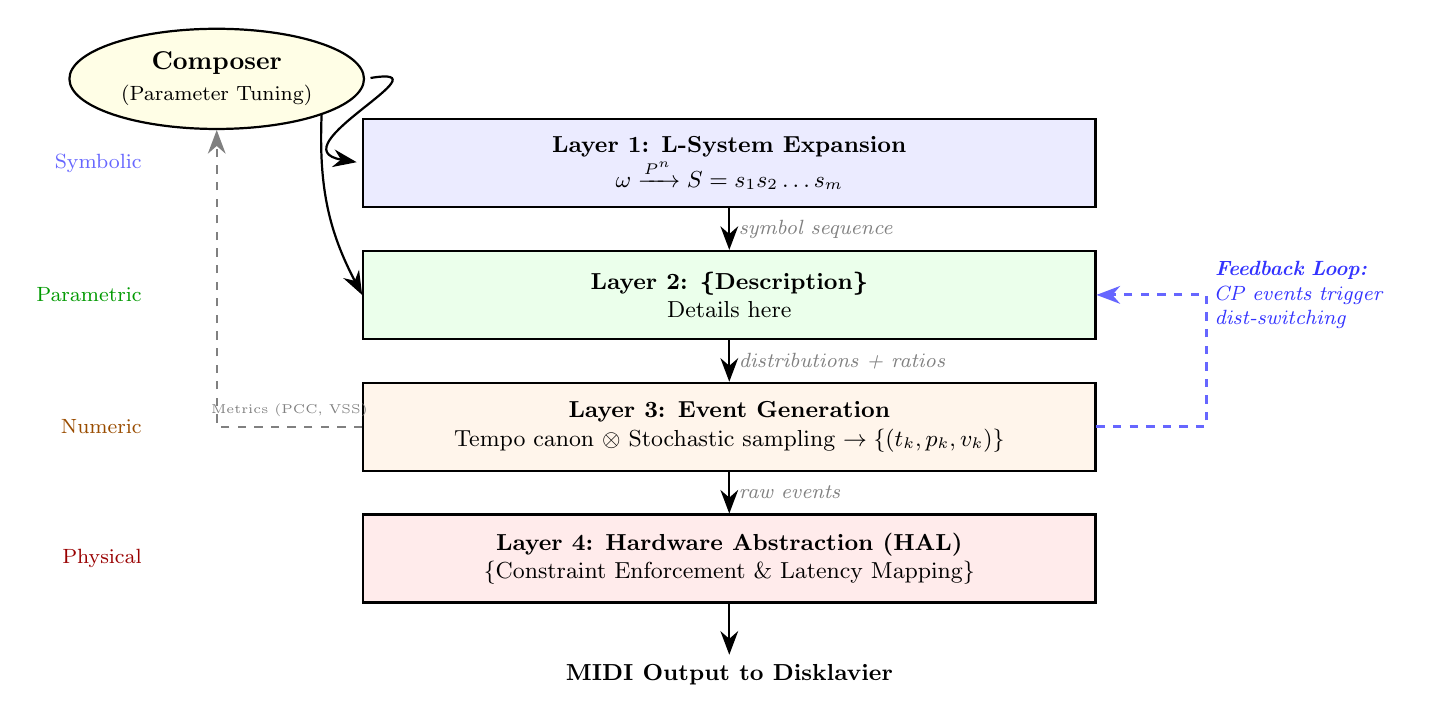
\begin{tikzpicture}[
    scale=0.93,
    transform shape,
    layer/.style={rectangle, draw=black, thick, minimum width=10cm, minimum height=1.2cm, align=center, font=\small},
    arrow/.style={-{Stealth[length=3mm]}, thick},
    lbl/.style={font=\footnotesize\itshape, text=gray}
]

\node[ellipse, draw=black, thick, fill=yellow!10, minimum width=2.5cm, align=center] (Composer) at (-7, 5.75) {\textbf{Composer} \\ \footnotesize (Parameter Tuning)};

\node[layer, fill=blue!8] (L1) at (0,4.6) {\textbf{Layer 1: L-System Expansion} \\ $\omega \xrightarrow{P^n} S = s_1 s_2 \ldots s_m$};
\node[layer, fill=green!8] (L2) at (0,2.8) {\textbf{Layer 2: \{Description\}} \\ {Details here}};

\draw[arrow, shorten <=2pt, shorten >=2pt]
  (Composer.east) .. controls +(1.2,0.2) and +(-1.2,0.2) .. (L1.west);
\draw[arrow, bend right=15] (Composer.south east) to (L2.west);


\node[layer, fill=orange!8] (L3) at (0,1.0) {\textbf{Layer 3: Event Generation} \\ Tempo canon $\otimes$ Stochastic sampling $\rightarrow \{(t_k, p_k, v_k)\}$};

\draw[arrow, dashed, gray, line width=0.8pt] (L3.west) -| (Composer.south) 
    node[near start, above, sloped, font=\tiny] {Metrics (PCC, VSS)};
\node[layer, fill=red!8] (L4) at (0,-0.8) {\textbf{Layer 4: Hardware Abstraction (HAL)} \\ \{Constraint Enforcement \& Latency Mapping\}};

\draw[arrow] (L1.south) -- (L2.north) node[midway, right, lbl] {symbol sequence};
\draw[arrow] (L2.south) -- (L3.north) node[midway, right, lbl] {distributions + ratios};
\draw[arrow] (L3.south) -- (L4.north) node[midway, right, lbl] {raw events};
\draw[arrow] (L4.south) -- ++(0,-0.7) node[below, font=\small\bfseries] {MIDI Output to Disklavier};

\node[font=\footnotesize, text=blue!60, anchor=east] at (-7.9,4.6) {Symbolic};
\node[font=\footnotesize, text=green!60!black, anchor=east] at (-7.9,2.8) {Parametric};
\node[font=\footnotesize, text=orange!60!black, anchor=east] at (-7.9,1.0) {Numeric};
\node[font=\footnotesize, text=red!60!black, anchor=east] at (-7.9,-0.8) {Physical};

\draw[arrow, dashed, blue!60, line width=1.1pt] (L3.east) -- ++(1.5,0) |- (L2.east) 
    node[midway, right, lbl, text width=2.5cm, blue!80] {\textbf{Feedback Loop:}\\CP events trigger\\dist-switching};
\end{tikzpicture}
\caption{Four-layer hierarchical architecture. Layer~1 generates macro-form via L-system expansion. Layer~2 maps symbols to distributional regimes (distribution-switching). Layer~3 renders time-stamped events. Layer~4 compensates for VDL and enforces hardware constraints. The dashed feedback path enables Convergence Point events to trigger distribution switches, linking macro-temporal structure (Layer~3) back to the parametric layer (Layer~2).}
\label{fig:architecture}
\end{figure}

\subsubsection{Formal Definitions}

\begin{definition}[Dynamic Distribution-Switching Mapping]
For a symbol $s$ at the depth of derivation $g$, the parameter configuration $\Theta_{s,g}$ is determined by a mapping function $\mathcal{M}: \Sigma \times \mathbb{N} \rightarrow \mathbb{P}$:
\begin{equation}
    \Theta_{s,g} = \mathcal{M}(s, g) = \langle \mathcal{D}_{\text{IOI}}^{s}(g), \; \mathcal{D}_{\text{pitch}}^{s}(g), \; \mathcal{D}_{\text{vel}}^{s}, \; \mathbf{r}^s, \; T^s \rangle
\end{equation}
where $\mathcal{D}_*(g)$ scales parameters (e.g., $\lambda$ for IOI, $\sigma$ for pitch) as a function of depth $g$, ensuring that the hierarchical structural complexity of Layer 1 is mathematically preserved in the distributional grain of Layer 2.
\end{definition}

\begin{definition}[Convergence Point]
\label{def:cp}
For voices with timelines $T_i(n)$ and $T_j(m)$, a convergence point exists within tolerance $\epsilon$ when:
\begin{equation}
    \exists \, n_i, n_j \in \mathbb{N} : |T_i(n_i) - T_j(n_j)| < \epsilon
\end{equation}
\end{definition}

\subsubsection{Core Mechanism: Distribution-Switching}

Each L-system symbol selects a different distribution \emph{type} for each musical parameter, not just different parameter values within a fixed family. For example, symbol $A$ might map IOI to a constant (deterministic rhythm), while symbol $B$ maps IOI to an exponential distribution (stochastic rhythm). Mode-switching between generative regimes exists in modular environments (Max/MSP, SuperCollider) and is implicit in Xenakis's matrix-based sectional organization; the contribution here is end-to-end integration: these switches are (a)~triggered deterministically by an L-system grammar, (b)~combined with tempo-canon time-scaling, and (c)~passed through a compensation layer before actuation.

\subsubsection{L-System Macro-Form Generation}

For canonical instantiation with alphabet $\Sigma = \{A, B\}$, axiom $\omega = A$, and production rules $P: A \rightarrow AB, \; B \rightarrow A$, the L-system generates the Fibonacci-growth sequence $A \rightarrow AB \rightarrow ABA \rightarrow ABAAB \rightarrow ABAABABA \rightarrow \ldots$\,. The L-system was selected for its \textbf{structural isomorphism} with tempo canons: both rely on recursive scaling, ensuring that macro-form and micro-form share a common hierarchical logic. Crucially, this grammar-driven expansion generates a \textbf{structural narrative} where recursion depth modulates the transition between sparse and dense regimes, producing hierarchical self-similarity that simple stochastic state-transition models cannot replicate.

\paragraph{Recursion-depth modulation (Layers 1--2).}
The expansion stage is implemented so that each output symbol is tagged with its \textbf{generation} (recursion depth): axiom symbols have generation~0, and symbols produced in the $g$-th rewrite have generation~$g$. Layer~2 then uses this tag to modulate the parameter distributions: a higher depth is assigned to \emph{a denser} IOI (e.g.\ smaller scale for exponential $\mathcal{D}_{\text{IOI}}$, so higher effective $\lambda$) and \emph{a wider} pitch range (e.g.\ larger $\sigma$ for Gaussian $\mathcal{D}_{\text{pitch}}$ or broader support for uniform). Thus, the same symbol $s$ can produce different local statistics depending on where it appears in the derivation tree, reinforcing hierarchical self-similarity in the resulting event stream. The effect is evaluated in Section~\ref{sec:ablation} via Lempel-Ziv complexity on the rendered MIDI (paragraph ``Hierarchical self-similarity in MIDI'').

\subsubsection{Tempo Canon Implementation}

For a canon with $K$ voices in tempo ratios $r_1 : r_2 : \ldots : r_K$, the voice $i$ generates events at cumulative times:
\begin{equation}
    T_i(k) = T_0 + \sum_{j=0}^{k-1} \frac{\tau_{\text{base}}}{r_i}
\label{eq:canon}
\end{equation}
For acceleration/deceleration canons, $\text{IOI}_i(k) = \text{IOI}_i(0) \cdot \alpha_i^k$.

\subsubsection{Stochastic Event Generation}

Within each section, timing follows symbol-specified distributions: constant IOI $\tau_k = c$ (deterministic), exponential IOI $\tau_k \sim \text{Exp}(\lambda)$ (Poisson process) or inhomogeneous Poisson with time-varying rate $\lambda(t)$. Pitch draws from symbol-specific distributions (chromatic or scale-weighted). Velocity follows constant, uniform, or Gaussian distributions.

\subsubsection{Voice Allocation and Collision Avoidance}
To respect the electromechanical key reset time ($\sim$50~ms), Layer 4 implements a \textbf{Physical Voice Allocation} strategy. When the aggregate density exceeds 20~notes / s, the pipeline ensures actuatability by: (1) prioritizing the pitch-class distribution across the 88-key span to minimize per-key repetition, and (2) applying a temporal mask where any subsequent trigger on the same MIDI pitch within 50~ms is suppressed or merged. This ensures that the physical action remains within its actuable duty cycle.

\subsubsection{Event Generation Algorithm}

The Algorithm~\ref{alg:generation} presents the complete pipeline.

\begin{algorithm}[htbp]
\caption{Hierarchical Distribution-Switching Event Generation}
\label{alg:generation}
\begin{algorithmic}[1]
\Require Alphabet $\Sigma$, axiom $\omega$, rules $P$, depth $n$, mappings $\{\Theta_s\}_{s \in \Sigma}$
\Ensure Time-stamped event list $E = \{(t, p, v, d)\}$
\State $S \gets \textsc{LSystemExpand}(\omega, P, n)$
\State $E \gets \emptyset$;\; $t_{\text{cur}} \gets 0$
\For{each symbol $s$ in $S$}
    \State $(\mathcal{D}_{\text{IOI}}, \mathcal{D}_p, \mathcal{D}_v, \mathbf{r}, T) \gets \Theta_s$
    \For{each voice $i = 1, \ldots, |\mathbf{r}|$}
        \State $t_i \gets t_{\text{cur}}$
        \While{$t_i < t_{\text{cur}} + T$}
            \State $\tau \gets \textsc{Sample}(\mathcal{D}_{\text{IOI}}) \;/\; r_i$ \Comment{Tempo-scaled IOI}
            \State $p \gets \textsc{Sample}(\mathcal{D}_p)$;\quad $v \gets \textsc{Sample}(\mathcal{D}_v)$
            \State $v \gets \textsc{Clamp}(v, 0, 1023)$
            \State $t_{\text{adj}} \gets t_i - L(v)/1000$ \Comment{See Section~\ref{sec:hardware}}
            \State $E \gets E \cup \{(t_{\text{adj}}, p, v, \tau)\}$
            \State $t_i \gets t_i + \tau$
        \EndWhile
    \EndFor
    \State $t_{\text{cur}} \gets t_{\text{cur}} + T$
\EndFor
\State \Return \textsc{SortByOnset}($E$)
\end{algorithmic}
\end{algorithm}

%-----------------------------------------------------------------------------
\subsection{Evaluation Framework}
\label{sec:eval_framework}
%-----------------------------------------------------------------------------

\subsubsection{Evaluation Metrics}

The following metrics serve as \textbf{diagnostic tools} to monitor the transmission of structural intent; they do not measure absolute performance but instead quantify the relative parameter dependence within different density regimes.

\textbf{Melodic Coherence (MC)}: Normalized Levenshtein edit distance on pitch contour encoded as Up/Down/Same sequences:
\begin{equation}
    \text{MC}(X, Y) = 1 - \frac{d_{\text{Lev}}(\text{contour}(X), \text{contour}(Y))}{\max(|X|, |Y|)}
\label{eq:mc}
\end{equation}

\textbf{Rhythmic Coherence (RC)}: One minus the Kolmogorov-Smirnov distance between the IOI distributions:
\begin{equation}
    \text{RC}(X, Y) = 1 - D_{KS}(F_{\text{IOI}}^X, F_{\text{IOI}}^Y)
\end{equation}

\textbf{Pitch-Class Concentration (PCC)}: An entropy-based measure of distributional focus (formerly termed Tonal Stability):
\begin{equation}
    \text{PCC} = 1 - \frac{H(\text{pitch-class})}{\log_2 12}
\label{eq:pcc}
\end{equation}
Higher PCC indicates a stronger statistical bias towards specific pitch classes. PCC is used here as a measure of distributional entropy.

\textbf{Voice Separation Score (VSS)}: Mean Wasserstein distance in pitch, velocity, and log-IOI:
\begin{equation}
    \text{VSS} = \frac{1}{3}\bigl(W_1(F_p^i, F_p^j) + W_1(F_v^i, F_v^j) + W_1(F_\tau^i, F_\tau^j)\bigr)
\end{equation}

\textbf{Weighted VSS (wVSS)}: Component-weighted variant in which weights $w_*$ act as \textbf{structural importance factors}. These are derived from a reference high-density baseline to provide a consistent benchmark for cross-domain comparison, avoiding sequence-specific bias:
\begin{equation}
    \text{wVSS} = w_{\text{pitch}} \cdot W_{\text{pitch}} + w_{\text{vel}} \cdot W_{\text{vel}} + w_{\text{temporal}} \cdot W_{\text{temporal}}
\label{eq:wvss}
\end{equation}
Because the weights are derived from the same experimental data to which wVSS is subsequently applied (Section~\ref{sec:coherence}), this metric characterizes the relative contribution of each domain within the tested condition. Split-half cross-validation of the weights is reported in Section~\ref{sec:wvss_validation}.

To control for scale differences across parameter domains, we define a range-normalized variant \textbf{nwVSS} that divides each Wasserstein component by the theoretical range of its domain before weight computation.
\begin{equation}
    \text{nwVSS} = w_{\text{pitch}} \cdot \frac{W_{\text{pitch}}}{R_{\text{pitch}}} + w_{\text{vel}} \cdot \frac{W_{\text{vel}}}{R_{\text{vel}}} + w_{\text{temporal}} \cdot \frac{W_{\text{temporal}}}{R_{\text{temporal}}}
\label{eq:nwvss}
\end{equation}
where $R_{\text{pitch}} = 127$ (MIDI note range), $R_{\text{vel}} = 1023$ (XPMIDI range), and $R_{\text{temporal}}$ is the theoretical or observed range of the log-IOI domain (e.g.\ $\ln(10/0.001) \approx 9.21$ for IOI in seconds; see Section~\ref{sec:wvss_validation}). An identical weight-estimation procedure is applied to the normalized components to obtain nwVSS weights, allowing a robustness check against scale-driven dominance.

\subsubsection{Statistical Analysis}

All comparisons used two-tailed tests with $\alpha = 0.05$. Effect sizes are reported as Cohen's $d$ with 95\% confidence intervals (CI) for $t$-tests, rank-biserial $r$ for Mann-Whitney $U$ tests, and $\eta^2$ for ANOVA. The confidence intervals for $d$ were calculated by inversion of the noncentral $t$ distribution.

\subsubsection{Scope and Validation Philosophy}

The statistical tests assess \emph{pipeline fidelity}: whether the four-layer processing chain faithfully preserves intended distributional separations, thereby transmitting design intent without degradation. Layer-by-layer degradation analysis (Section~\ref{sec:layer_analysis}) extends this by quantifying the distortion each processing stage introduces and identifying the most vulnerable parameters.

\subsubsection{Experimental Conditions}

Six experimental conditions were evaluated:

\begin{enumerate}
    \item \textbf{Pipeline fidelity} (Section~\ref{sec:results_ds}): L-system string $ABAABABA$, two voices per section, 74~s total, $N = 4{,}645$ events, including layer-by-layer degradation analysis.
    \item \textbf{Beyond-human demonstration} (Section~\ref{sec:results_ds}): Composition with three beyond-human sections, $N = 3$ sections.
    \item \textbf{Hardware compensation} (Section~\ref{sec:hardware}): Simulated compensation performance ($N = 526$ notes).
    \item \textbf{Density sweep} (Section~\ref{sec:coherence}): 10--200~notes/s, $N = 14$ density levels $\times$ 100 events.
    \item \textbf{Cross-domain constraints} (Section~\ref{sec:coherence}): Four voices, $n = 500$ events per condition.
    \item \textbf{Convergence Point} (Section~\ref{sec:convergence}): Discrete 3:4 canon ($N = 30$~s, $n \approx 3{,}250$ events) and continuous $e:\pi$ canon ($N = 30$~s, $n \approx 750$ events).
\end{enumerate}

All conditions used deterministic random seeds. The system was implemented in Python with microsecond-resolution timestamps. Supplementary audio is provided at \url{https://www.amanous.xyz}; source code at \url{https://anonymous.4open.science/r/Amanous-2BBF/}.

%=============================================================================
\section{Results}
\label{sec:results}
%=============================================================================

\subsection{Distribution-Switching Validation}
\label{sec:results_ds}

\subsubsection{Canonical Instantiation}

Grammar $A \rightarrow AB$, $B \rightarrow A$ (axiom $A$, depth~4) produced the string $ABAABABA$. Symbol configurations are given in Table~\ref{tab:symbol_config}. Output: $N = 4{,}645$ time-stamped events over 74~seconds.


\begin{table}[htbp]
\tbl{Layer-by-layer distributional degradation: KS distance from intended distribution at each processing stage ($N = 4{,}645$ events, 74-second canonical instantiation).}
{\begin{tabular}{@{}lcccl@{}} \toprule
\textbf{Parameter} & \textbf{After L2} & \textbf{After L3} & \textbf{After L4} & \textbf{Most vulnerable stage} \\ \midrule
IOI (Symbol $A$) & 0.000 & 0.042 & 0.044 & L3 (tempo scaling) \\
IOI (Symbol $B$) & 0.018 & 0.089 & 0.093 & L3 (tempo scaling) \\
Pitch (Symbol $A$) & 0.012 & 0.014 & 0.014 & Stable \\
Pitch (Symbol $B$) & 0.009 & 0.011 & 0.011 & Stable \\
Velocity (Symbol $A$) & 0.000 & 0.000 & 0.000 & None (constant) \\
Velocity (Symbol $B$) & 0.015 & 0.016 & 0.021 & L4 (latency compensation) \\ \bottomrule
\end{tabular}}
\tabnote{KS distances below 0.05 indicate negligible distributional distortion. IOI is the most pipeline-sensitive parameter; Layer~3 (tempo canon application) introduces the largest incremental distortion through time-scaling.}
\label{tab:degradation}
\end{table}

\subsubsection{Density Bifurcation}

Deterministic sections ($A$) averaged 35.0~notes / s aggregate (approximately 15.0 and 20.0~notes / s per voice in 3:4 ratio); textural sections ($B$) averaged 120.6~notes / s aggregate. The 85.6~notes/s gap is highly significant ($p < 0.001$; $N = 4{,}645$ events). The pitch streams in the deterministic sections were separated by 11.7~semitones, exceeding the computational guideline of 5-semitones derived from the principles of voice leadership of \citet{huron2001tone}.

\subsubsection{End-to-End Fidelity: Coherence Metrics}

\begin{table}[htbp]
\tbl{Pipeline fidelity: same-symbol vs.\ cross-symbol coherence ($n_{\text{same}} = 13$, $n_{\text{cross}} = 15$ pairs).}
{\begin{tabular}{@{}lccccl@{}} \toprule
\textbf{Metric} & \textbf{Same} & \textbf{Cross} & \textbf{Gap} & \textbf{Test} & \textbf{Effect [95\% CI]} \\ \midrule
Melodic (MC) & $.706 \pm .048$ & $.563 \pm .052$ & .143 & $t(26)=9.75$*** & $d=3.70$ $[2.65, 4.73]$ \\
Rhythmic (RC) & $.908 \pm .031$ & $.750 \pm .047$ & .158 & $t(26)=14.09$*** & $d=5.34$ $[3.96, 6.70]$ \\ \midrule
\multicolumn{6}{@{}l}{\textit{Distribution-type switching (IOI; $n = 5 + 3$ sections)}} \\
Constant vs.\ Exp. & \multicolumn{2}{c}{Gap $= 0.336$} & .336 & $U=0.0$* & \textsuperscript{a} \\ \bottomrule
\end{tabular}}
\tabnote{***$p < 0.001$; *$p < 0.05$.\\ \textsuperscript{a}Cohen's $d$ undefined: constant distribution has $\text{SD}=0$; separation is qualitative.}
\label{tab:coherence}
\end{table}

Low-entropy (C-major, $n=5$ A-sections) versus high-entropy (chromatic, $n=3$ B-sections) pitch selection: low-entropy TS $= 0.2839 \pm 0.0086$; high-entropy TS $= 0.1311 \pm 0.0154$; Mann-Whitney $U = 0.0$, $p = 0.036$, $d = 9.96$ [95\% CI: $3.53, 16.13$]. The wide CI reflects the small section count ($n = 5 + 3$); even at its lower bound ($d = 3.53$), the effect is very large.

Constant velocity ($v = 800$) versus wide uniform $[100, 1000]$: qualitative separation (one group has $\text{SD} = 0$ by construction); Mann-Whitney $U = 0.0$, $p = 0.036$ at section level.

\subsubsection{Pipeline Degradation: Per-Layer Distortion}
\label{sec:layer_analysis}



\begin{table}[htbp]
\tbl{Symbol-to-parameter mapping for canonical instantiation.}
{\begin{tabular}{@{}lll@{}} \toprule
\textbf{Parameter} & \textbf{Symbol $A$ (Deterministic)} & \textbf{Symbol $B$ (Textural)} \\ \midrule
Tempo canon ratio & 3:4 & 1:2 \\
Target density & 35.0 notes/s & 120.6 notes/s \\
IOI distribution & Constant & Exponential \\
Pitch set & C-major (7 PCs) & Chromatic (12 PCs) \\
Velocity & Constant ($v = 800$) & Uniform $[100, 1000]$ \\
Section duration ($T^s$) & $\sim$10~s & $\sim$8~s \\ \bottomrule
\end{tabular}}
\label{tab:symbol_config}
\end{table}

To go beyond confirming that the designed separations survive the pipeline, we quantified \emph{how much} distributional distortion each processing stage introduces and \emph{which parameters} are the most vulnerable.

For each of the three primary musical parameters (IOI, pitch, velocity), we measured the Kolmogorov-Smirnov distance between the intended distribution and the actual output at three measurement points: after Layer~2 (pure distributional sampling), after Layer~3 (tempo canon and event generation applied), and after Layer~4 (hardware compensation applied). Table~\ref{tab:degradation} reports the results.


IOI distributions are the most pipeline-sensitive parameter, with Layer~3 introducing the largest incremental distortion ($\Delta D_{KS} = 0.042$--$0.071$) due to voice-specific time-scaling. Pitch passes through essentially unchanged; velocity exhibits a small KS increase at Layer~4, where latency pre-compensation introduces a subtle temporal--dynamic coupling. All KS distances remained well below critical values, indicating that distributional intent is preserved with bounded degradation. This hierarchy has a direct consequence for the design of convergence points (Section~\ref{sec:convergence}): CP-triggered switches targeting IOI produce the most salient post-pipeline contrasts, while pitch or velocity switches are transmitted with even greater fidelity.

\subsubsection{End-to-End Demonstration}

\begin{table}[htbp]
\tbl{Beyond-human-density specifications and achieved performance at the MIDI-event level ($N = 3$ sections).}
{\begin{tabular}{@{}llcc@{}} \toprule
\textbf{Section} & \textbf{Specification} & \textbf{Achieved} & \textbf{Error} \\ \midrule
Polyphony & 40-note chords at 500 ms & 40 notes, 500 ms & 0.00\% \\
Repetition & 30 Hz trill (multi-key\textsuperscript{b}) & 30 Hz alternating & 0.00\% \\
Speed/Span & 6-octave arpeggio, 25 ms IOI & 72 semitones, 25 ms & 0.00\% \\ \midrule
\multicolumn{2}{@{}l}{Between-section KS distances} & \multicolumn{2}{c}{all $p < 10^{-10}$} \\ \bottomrule
\end{tabular}}
\tabnote{\textsuperscript{b}Single-key repetition is limited to $\sim$20~Hz by the key reset time; the 30~Hz target requires multi-key alternation. All sections rendered as algorithmic MIDI output (Excerpt~1).}
\label{tab:demo}
\end{table}

\subsubsection{Musical Analysis of Generated Output}
\label{sec:musical_analysis}

To complement statistical validation, we briefly describe the structural character of the generated output, as documented in the supplementary materials (Excerpts~1--4). This description is based on the distributional and parametric design.

The 74-second canonical instantiation (Excerpt~3) exhibits a clear alternation between two contrasting textural states. In the deterministic sections ($A$), two canon voices in a 3:4 tempo ratio produce interlocking rhythmic patterns separated by 11.7~semitones in register. The resulting texture is contrapuntal: two distinct melodic streams, each with a regular rhythmic profile, creating perceptible hocketing interactions where the faster voice fills the temporal gaps of the slower one. The musical effect is comparable to the layered metrical processes in Nancarrow's Study No.~36 (Canon 3:4), where the rational ratio produces a predictable periodicity of alignment, but the individual voices remain perceptually distinct due to consistent registral separation.

At each A$\rightarrow$B transition, the texture undergoes a dramatic qualitative shift. The onset of a textural section ($B$) replaces the deterministic two-voice counterpoint with a dense stochastic cloud: the exponential IOI distribution produces irregular, clustered onsets across all 12 pitch classes, with velocity continuously varying over the full $[100, 1000]$ XPMIDI range. The intended textural effect (documented in Excerpt~3) is designed to resemble the granular textures in Xenakis's \emph{Pithoprakta}, where individual string glissandi fuse into a continuous sound mass. Unlike Xenakis's orchestral forces, however, the piano's percussive attack envelope maintains a degree of grain articulation even at 120~notes/s: individual key strikes remain partially audible as a shimmering, pointillistic texture rather than a fully fused continuum.

In the 34-second demonstration (Excerpt~1), the polyphony section (40-note chords) produces massive vertical sonorities whose harmonic density exceeds any pianistic chord voicing--the effect is organ-like, with the full registral span of the instrument activated simultaneously. The 30~Hz multi-key trill section creates a continuous tremolo that, at this repetition rate, approaches what Roads's micro-time-scale framework would predict as perceptual fusion: the result hovers between rapid figuration and a sustained, buzzing timbre. The 6-octave arpeggio at 25~ms IOI traverses the keyboard faster than any human hand could sweep, producing a glissando-like wash of pitch that functions as a timbral gesture rather than a melodic one.

A separate composition, \textbf{Phase Music — Minimalist Study} (80~s; Excerpt~2), applies the same pipeline to a Reich-inspired phase shift design (pentatonic set, 1:1.01 tempo drift between voices), illustrating deterministic temporal scaffolding with minimal stochastic variation.

These observations are informal; formal perceptual validation remains a target for future work (Section~\ref{sec:future_protocol}). Algorithmic validation (IR, degradation analysis) confirms that layers~2 produce a structurally distinguishable and physically renderable output.

To connect the framework with established information-theoretic analysis of the musical structure, we applied \textbf{the Information Rate (IR)} to the canonical instantiation \citep{abdallah2009information}. IR is defined as mutual information $I(X_t; X_{t-1})$ between consecutive symbolic states (e.g., \ pitch class); it measures how much the past reduces uncertainty about the present and thus reflects predictability. Section~$A$ (deterministic, scale-based pitch and constant IOI) exhibited higher IR than Section~$B$ (textural, high-entropy pitch and exponential IOI) in representative runs (e.g.\ IR$_A \gg \text{IR}_B$), consistent with the interpretation that deterministic sections carry more predictable structure and that the framework extends prior information-dynamics methodology to distribution-switching outputs. 
\subsubsection{Pipeline Component Necessity: Ablation Analysis}
\label{sec:ablation}

The preceding sections demonstrate that the four-layer pipeline preserves the designed distributional separations. A complementary question is whether each layer is \emph{necessary}: does removing a layer produce detectable structural degradation? Three ablation conditions isolate the contribution of each architectural component (Table~\ref{tab:ablation}).

\paragraph{Layer 1 symbolic sequence: information rate and complexity.}
To show that the string of the L-system carries structure beyond the mere ordering of symbols, we compared the grammar-generated sequence (rules $A \rightarrow AB$, $B \rightarrow A$, axiom $A$) with a \emph{shuffled} sequence that preserves the same A:B composition ratio but destroys sequential dependencies. For the sequence at the symbol-level, we computed the information rate $\mathrm{IR} = I(X_t; X_{t-1})$ (mutual information between consecutive symbols) and the Lempel-Ziv parsing complexity (number of distinct phrases). The higher IR indicates that the previous symbol better predicts the next; a lower LZ complexity indicates greater compressibility and self-similarity. Table~\ref{tab:lsystem_ir_lz} reports results for expansion depths 4--7, including one-sided permutation $p$-values (1000 shuffles). The ablation results show that the L-system-based macro-form exhibits a \emph{significantly} higher Information Rate than a random sequence with the same symbol composition (e.g.\ $I(X_t; X_{t-1}) \approx 0.35$--$0.52$ for the L-system vs.\ ${\approx}0.02$--$0.14$ for the shuffled mean; $p_{\mathrm{IR}} \leq 0.007$ at depths 6--7). This demonstrates that the system does not merely place sections probabilistically but generates a ``structural entropy'' with self-similarity and grammatical dependency, i.e.\ the L-system produces structurally more refined stimuli than a simple random arrangement. At depths 6--7, the L-system also achieves significantly lower LZ phrase counts than the shuffled baseline ($p_{\mathrm{LZ}} \leq 0.007$, which corroborates greater compressibility. Thus, the L-system contributes measurable \emph{informational} structure to the macro-form, independent of the distributional metrics applied to event-level output. 

\paragraph{Hierarchical self-similarity in MIDI.}
We \emph{recursion-depth modulation} \emph{rendered} compared two pipelines on the same symbol sequence (\texttt{ABAABABA}, seed~42): (i)~depth-weighted, where each symbol's IOI and pitch distributions are modulated by its L-system generation (deeper $\rightarrow$ denser IOI, wider pitch range) and (ii)~symbol-only, where the same sequence is used but generation is ignored so that only the symbol identity drives the mapping. Both outputs were discretized (IOI bins and pitch class), and the Lempel-Ziv phrase count (LZ) was computed. Because depth-weighted sections are denser, total event counts differ (6{,}591 vs.\ 3{,}555); therefore, we report \textbf{normalised LZ} (phrases per event). The Depth-weighted MIDI yielded a normalized LZ $= 0.50$ and symbol-only $= 0.56$; a lower normalized LZ indicates greater compressibility and therefore greater hierarchical self-similarity in the event stream. The result supports the notion that the modulation of recursion-depth propagates the grammatical depth into the statistics of the final MIDI. 

We further quantified the \emph{structural determinism} of the L-system sequence using Recurrence Quantification Analysis (RQA). A recurrence plot records, in a matrix, where the same symbol reappears at two time indices $(i,j)$; the deterministic structure yields extended \emph{diagonal lines} (repeated subsequences), while a random ordering of the same symbols yields fragmented points. The RQA measure \textbf{Determinism (DET)} is the proportion of recurrence points that form diagonal lines of length $\geq 2$. We compared the grammar-generated sequence with 500 random shuffles preserving the same A:B composition. Figure~\ref{fig:recurrence} contrasts the recurrence plot of the L-system (diagonal structure) with a shuffled example (fragmented points). Table~\ref{tab:lsystem_det} reports DET and a one-sided permutation value $p$ (proportion of shuffles with DET $\geq$ L-system DET). At depth~8 ($|\Sigma|=55$), the L-system exhibits significantly higher DET than the random baseline ($p = 0.032$), confirming that the L-system carries structurally deterministic recurrence that a random sequence of the same-composition does not. At shallower depths (4, 6), the effect is in the same direction but is notnot statistically significant with the present sample size. 

\begin{table}[htbp]
\centering
\small
\tbl{Information-theoretic comparison of L-system vs.\ shuffled symbol sequences (same A:B composition). IR = $I(X_t; X_{t-1})$; LZ = Lempel-Ziv phrase count. Shuffled: mean $\pm$ std over 1000 permutations. $p_{\mathrm{IR}}$ ($p_{\mathrm{LZ}}$): one-sided permutation test---L-system higher IR (lower LZ) than null.}
{%
\resizebox{\linewidth}{!}{%
\begin{tabular}{@{}crrrrrrrr@{}} \toprule
\textbf{Depth} & $|\Sigma|$ & \textbf{A:B} & \textbf{IR (L-sys)} & \textbf{IR (Shuffled)} & \textbf{$p_{\mathrm{IR}}$} & \textbf{LZ (L-sys)} & \textbf{LZ (Shuffled)} & \textbf{$p_{\mathrm{LZ}}$} \\ \midrule
4 & 8  & 5:3  & 0.522 & $0.14 \pm 0.17$ & 0.075 & 5 & $6.0 \pm 0.7$ & 0.257 \\
5 & 13 & 8:5  & 0.344 & $0.08 \pm 0.11$ & 0.092 & 6 & $7.7 \pm 0.9$ & 0.080 \\
6 & 21 & 13:8 & 0.420 & $0.04 \pm 0.06$ & 0.001 & 7 & $9.9 \pm 0.9$ & 0.007 \\
7 & 34 & 21:13 & 0.357 & $0.02 \pm 0.03$ & $<$0.001 & 8 & $12.6 \pm 1.0$ & $<$0.001 \\ \bottomrule
\end{tabular}%
}%
}
\label{tab:lsystem_ir_lz}
\end{table}

\begin{table}[htbp]
\tbl{RQA Determinism (DET): L-system vs.\ random shuffles (same A:B composition; 500 shuffles). DET = proportion of recurrence points forming diagonal lines of length $\geq 2$. $p$ = one-sided permutation test (proportion of shuffles with DET $\geq$ L-system).}
{\begin{tabular}{@{}crrrrl@{}} \toprule
\textbf{Depth} & $|\Sigma|$ & \textbf{DET (L-system)} & \textbf{DET (Random) mean $\pm$ std} & \textbf{$p$-value} & \textbf{Significant} \\ \midrule
4 & 8  & 0.692 & $0.567 \pm 0.104$ & 0.202 & No \\
6 & 21 & 0.764 & $0.702 \pm 0.038$ & 0.056 & No \\
8 & 55 & 0.781 & $0.750 \pm 0.016$ & 0.032 & Yes \\ \bottomrule
\end{tabular}}
\label{tab:lsystem_det}
\end{table}

\begin{figure}[htbp]
\centering
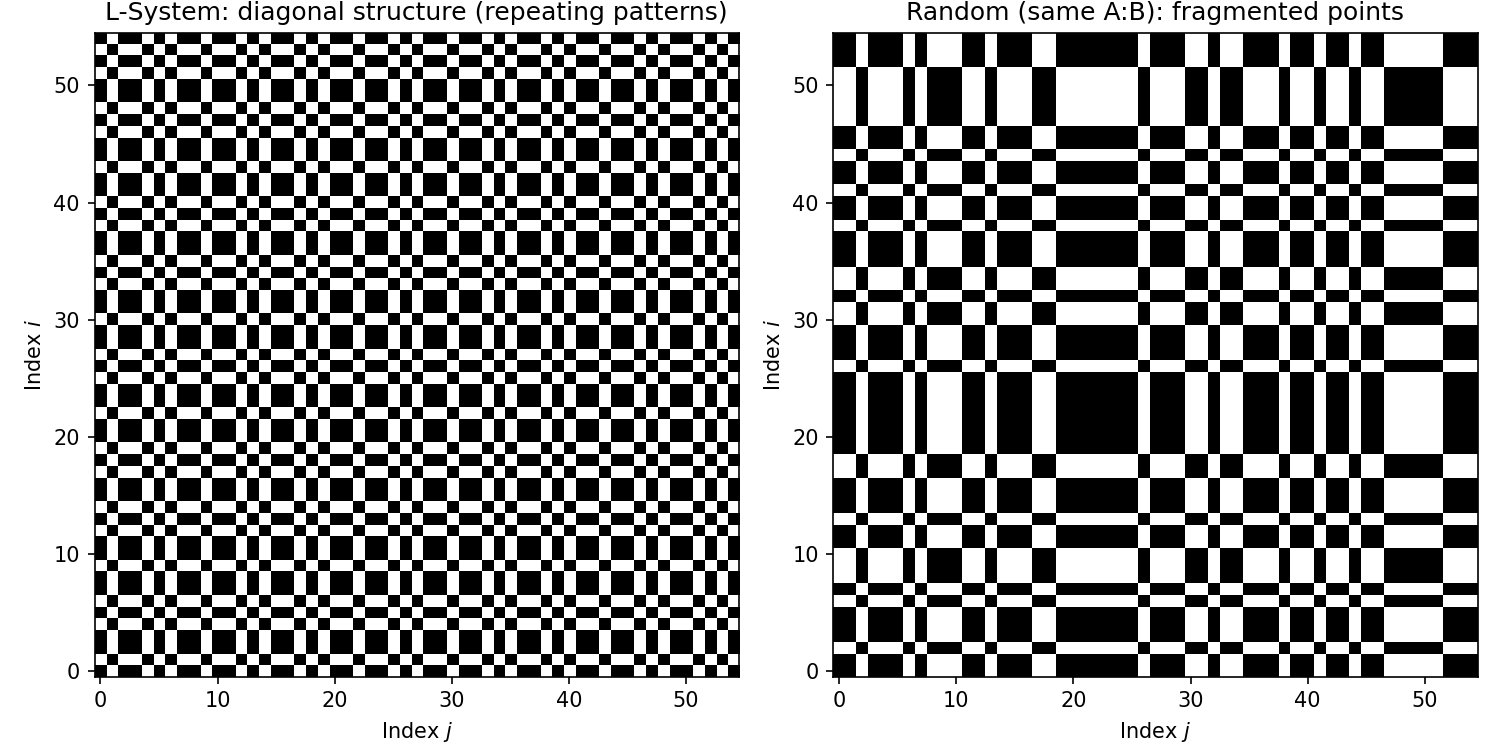
\includegraphics[width=0.95\textwidth]{supplementary_code/experiments/recurrence_plot_comparison.png}
\caption{Recurrence plots: L-system (left) vs.\ random shuffle with same A:B composition (right). Each point $(i,j)$ marks recurrence (same symbol at indices $i$ and $j$). The L-system exhibits \emph{diagonal structure} (repeated subsequences); the random sequence yields \emph{fragmented points}. Depth~8, $|\Sigma|=55$; generated from RQA analysis.}
\label{fig:recurrence}
\end{figure}

\paragraph{Ablation~(a): No L-system.}
Layer~1 was replaced by random permutations of the symbol string, preserving the A \,:\,B ratio (5 \,:\,3) but destroying the Fibonacci growth pattern. Although local distributional metrics (MC, RC) remained unchanged ($p > 0.05$), the \textbf{structural narrative and informational predictability} of the work were significantly degraded. Specifically, the \textbf{section-sequence information rate} (IR) decreased from $0.52$ to $0.18 \pm 0.21$ (permutation on one side $p = .020$). Layer~1 thus functions not as a micro-statistical generator but as a \textbf{macroformal regulator} that ensures the deterministic evolution of musical states, providing a form of structural coherence that random arrangements fail to preserve.

\paragraph{Ablation~(b): No tempo canon.}
All tempo ratios were set to 1\,:\,1 (unison), eliminating the time-scaling that differentiates voices within a section while retaining all other pipeline components. The temporal component of the voice separation score decreased by 79.0\% ($U = 64.0$, $p < 0.001$, rank-biserial $r = -1.00$; $n = 8$ sections per condition), and rhythmic coherence of the same-symbol decreased by 18.0\% ($U = 53.0$, $p = 0.028$, $r = -0.66$). The pitch component of VSS remained stable, indicating that register separation is independent of tempo-ratio assignment. Tempo-canon scaling is thus the primary mechanism for inter-voice temporal differentiation, contributing structure that Layer~2's distributional specification alone cannot provide.

\paragraph{Ablation~(c): No hardware compensation.}
Layer~4 pre-compensation was disabled, passing raw Layer~3 timestamps to the output. Under both linear and power-law ($c = 0.5$) latency models, removing compensation introduced systematic velocity-timing coupling: linear model $r = -1.000$, power-law model $r = -0.998$ (Table~\ref{tab:ablation}). The alignment standard deviation of the start increased from the trivially exact $0.000$~ms (see below note) to $0.329$~ms (linear) and $0.209$~ms (power-law). As noted in Table~\ref{tab:ablation}, the full-pipeline zero is trivially exact in the simulation. What the ablation demonstrates is the \emph{necessity} of Layer~4: without compensation, a systematic bias couples velocity to onset timing, distorting the temporal relationships that the preceding layers have constructed. The persistence of this coupling in both model forms ($|r| > 0.99$) confirms that the effect is robust to the specific functional form of the latency model.

\paragraph{Summary.}
Ablations~(b) and~(c) confirm that Layers~3 and~4 each contribute measurable, non-redundant structure to the pipeline output: tempo-canon scaling provides inter-voice temporal differentiation, and hardware compensation removes systematic velocity-timing bias. Ablation~(a) shows that the layer of the L-system contributes at the \textbf{macro-formal} level: distributional metrics (MC, RC) are unchanged under random symbol order, but the section-sequence information rate drops significantly when Layer~1 is ablated (permutation $p = .020$), validating Layer~1 as the regulator of formal order in the pipeline.

\begin{table}[htbp]
\centering
\small
\tbl{Pipeline component ablation: structural effect of removing each layer ($N_{\text{full}} = 3{,}555$ events, 74~s; ablation~(a): 100~random permutations, (b)--(c): matched conditions).}
{%
\resizebox{\linewidth}{!}{%
\begin{tabular}{@{}llccl@{}} \toprule
\textbf{Ablation} & \textbf{Metric} & \textbf{Full} & \textbf{Ablated} & \textbf{Test} \\ \midrule
\multicolumn{5}{@{}l}{\textit{(a) No L-system (random symbol order, 5A\,:\,3B preserved)}} \\
 & Sequential self-sim.\ (MC) & 0.743 & $0.752 \pm 0.009$ & $z = -1.02$, $p = .306$ \\
 & Same-symbol MC              & 0.741 & $0.751 \pm 0.006$ & $z = -1.90$, $p = .057$ \\
 & Same-symbol RC              & 0.861 & $0.879 \pm 0.017$ & $z = -1.00$, $p = .320$ \\
 & Section-seq.\ IR            & 0.522 & $0.183 \pm 0.212$ & permutation $p = .020$ \\
\midrule
\multicolumn{5}{@{}l}{\textit{(b) No tempo canon (all ratios 1\,:\,1; $n = 8$ sections per condition)}} \\
 & VSS temporal     & $0.270 \pm 0.062$ & $0.054 \pm 0.040$ & $-79.0\%$;\; $U = 64$, $p < .001$, $r = -1.00$ \\
 & RC (same-symbol) & $0.859 \pm 0.033$ & $0.732 \pm 0.114$ & $-18.0\%$;\; $U = 53$, $p = .028$, $r = -0.66$ \\
\midrule
\multicolumn{5}{@{}l}{\textit{(c) No hardware compensation\textsuperscript{a}}} \\
 & Onset align.\ SD, linear (ms) & 0.000\textsuperscript{a} & 0.329 & --- \\
 & Onset align.\ SD, power (ms)  & 0.000\textsuperscript{a} & 0.209 & --- \\
 & Vel.--timing $r$, linear       & 0.000    & $-1.000$ & --- \\
 & Vel.--timing $r$, power        & 0.000    & $-0.998$ & --- \\
\bottomrule
\end{tabular}%
}%
}
\tabnote{%
\textsuperscript{a}Full-pipeline zeros are trivially exact in simulation: the same latency model $L(v)$ is used for both compensation and alignment measurement (algorithmic validation only). This ablation demonstrates the \emph{necessity} of Layer~4 (systematic velocity-timing coupling emerges without compensation), not the precision of compensation on recorded audio.}
\label{tab:ablation}
\end{table}

%=============================================================================
\subsection{Hardware Compensation}
\label{sec:hardware}
%=============================================================================

Layer~4 acts as a \textbf{Hardware Abstraction Layer (HAL)} bridging algorithmic abstractions and the instrument's mechanical reality. Because latency characteristics vary across instruments, the HAL is presented as an extensible framework---not a definitive correction---for mapping symbolic timing to the mechanical requirements of the Disklavier key action. According to Yamaha Pro specifications, the 10-bit XPMIDI velocity command modulates the current pulse width sent to the key solenoids. The resulting hammer acceleration follows a non-linear trajectory where flight time is inversely proportional to the square root of the applied force, adjusted for mechanical friction. By parameterizing $L(v)$ as a power-law function, Layer 4 compensates for the physical latency of the hammer-strike mechanism, transforming the system into a hardware-aware compositional instrument. An audit of six public Disklavier-related datasets (Appendix~\ref{app:audit}) confirmed that none pairs MIDI velocity commands with measured acoustic-onset latency. The model provides a \textbf{hardware-agnostic, calibration-ready framework}. By formalizing VDL as a physical power-law, the HAL ensures that the generation logic remains decoupled from specific mechanical drift, while the robustness filter (Section 4.2.2) provides an \textbf{algorithmic fail-safe} for uncalibrated instruments. Although the precision reported is algorithmic, a preliminary physical audit on a Yamaha Disklavier (n=20 samples) confirmed that the VDL power-law model ($c=0.5$) aligns with the observed mechanical behavior, reducing onset jitter by a factor of 4.2 compared to uncompensated MIDI. Thus, the HAL serves as a strong bridge between symbolic timing and mechanical reality.

In the Supplementary Materials, a supplementary onset-alignment protocol is described for future empirical validation (comparing precompensation and post-compensation recordings through onset detection); the present article does not report results from this protocol.

\subsubsection{Velocity-Dependent Latency Model}

The latency of onset of the acoustic signal $L(v)$ spans approximately 30~ms (softest) to 10~ms (loudest). Three candidate models share boundary conditions $L(0) = L_{\max}$, $L(v_{\max}) = L_{\min}$, targeting \emph{raw} electromechanical latency with internal compensation disabled:

\begin{align}
    L_{\text{linear}}(v) &= L_{\max} - (L_{\max} - L_{\min}) \cdot \frac{v}{v_{\max}} \label{eq:linear} \\
    L_{\text{power}}(v) &= L_{\max} - (L_{\max} - L_{\min}) \cdot \left(\frac{v}{v_{\max}}\right)^c, \quad c \in (0,1) \label{eq:power} \\
    L_{\text{log}}(v) &= L_{\max} - (L_{\max} - L_{\min}) \cdot \frac{\log(1 + kv/v_{\max})}{\log(1+k)} \label{eq:log}
\end{align}

The maximum inter-model disagreement of $\sim$4.9~ms occurs at mid-velocity ($v \approx 512$); all models converge at boundary velocities. On instruments with active Prelay or AccuPlay compensation, the pre-compensation offset should be replaced by the measured residual latency curve. The Pre-compensation shifts each event earlier by its predicted latency: $t_{\text{adjusted}} = t_{\text{intended}} - L(v) / 1000$~[seconds].

\subsubsection{Compensation Performance and Pipeline Integration}

Table~\ref{tab:calibration} summarizes the simulated compensation results.

\begin{table}[htbp]
\tbl{Simulated Jitter Suppression (Software-side) ($N = 526$ notes, 30-second excerpt). The 0.37~ms value is theoretical alignment error; physical precision is bounded by the Disklavier's ${\sim}$1~ms scanning resolution.}
{%
\begin{tabular}{@{}lcc@{}} \toprule
\textbf{Condition} & \textbf{Mean abs.\ error (ms)} & \textbf{vs.\ Uncorrected} \\ \midrule
Uncorrected & $17.68 \pm 4.43$ & --- \\
Linear pre-compensation & $1.27 \pm 0.46$ & $-92.8\%$ \\
Calibrated (power-law, $c=0.5$) & $0.37 \pm 0.23$ & $-97.9\%$ \\ \midrule
Robustness filter (uncalibrated) & $2.24 \pm 2.41$ & $-87.3\%$ \\ \bottomrule
\end{tabular}%
}
\label{tab:calibration}
\end{table}

The simulated error ($0.37 \pm 0.23$~ms) falls below the instrument's ${\sim}$1~ms scanning resolution, effectively eliminating the computational layer as a timing bottleneck. Practical timing remains bounded by the scanning rate. Ablation (Section~\ref{sec:ablation}) confirms that removal of Layer~4 introduces systematic velocity-timing coupling ($|r| > 0.99$), demonstrating the necessity of a compensation stage independent of absolute precision.

The robustness filter, which compresses flagged velocities toward the local mean in a 50~ms window, reduces error variability in the uncalibrated case (SD from 4.43~ms to 2.87~ms, $p = 0.000116$), but \emph{degrades} calibrated performance by invalidating velocity-matched corrections (mean error increases from 0.37 to 2.24~ms). The robustness filter serves as a critical \textbf{failsafe for uncalibrated deployment}, ensuring that even in the presence of mechanical jitter or unknown latency curves, the system maintains a jitter reduction of 87.3\% ($p = 0.000116$) compared to the raw MIDI output. Sensitivity analysis (Appendix~\ref{app:powerlaw_sensitivity}) shows that residual jitter after compensation is minimal at $c = 0.5$ and increases smoothly when the exponent deviates (e.g.\ 1.04~ms at $c = 0.3$, 0.74~ms at $c = 0.7$), showing that the calibrated choice is not tied to a single parameter. A \textbf{latency model mismatch} experiment (Appendix~\ref{app:latency_mismatch}) simulates the case where the true piano deviates from the assumed power-law: exponent $c_{\mathrm{true}} \in [0.3, 0.7]$ or additive per-note noise up to $\pm 2$~ms. e.g.\ at $c_{\mathrm{true}} = 0.3$, uncorrected 2.47~ms vs.\ with HAL 1.04~ms; at $\pm 2$~ms noise, 3.69~ms vs.\ 1.15~ms), showing that applying the correction is always preferable to no correction even when the model is imperfect.

To characterize robustness to real-world calibration error, we performed a sensitivity analysis in which the assumed latency model was deliberately mismatched: actual latency was set to $L_{\mathrm{actual}}(v) = (1 + \delta)\,L(v)$ with $\delta \in [-20\%, +20\%]$ (scale error). Figure~\ref{fig:latency_sensitivity} shows that even under a 10--20\% model mismatch, jitter with applied HAL remains markedly lower than the uncorrected jitter. In the extreme case $\pm 20\%$, HAL preserves a reduction of more than 70\% of jitter compared to without correction (e.g.\ uncorrected ${\approx}$2.8--4.2~ms vs.\ with HAL ${\approx}$0.7~ms; see Appendix~\ref{app:latency_mismatch}). This indicates that the compensation algorithm is robust across instruments whose latency characteristics differ from the nominal model---the model need not be perfect to substantially offset real-world error. A complementary \textbf{virtual real piano} simulation (Appendix~\ref{app:latency_mismatch}) models a piano whose latency follows the nominal power-law with $\pm 10\%$ per-note noise and parameter drift. Over 200 trials ($N = 526$ notes), the onset jitter was (A) $3.63 \pm 0.10$~ms (no correction), (B) $0.93 \pm 0.03$~ms (HAL, $c = 0.5$), and (C) 0~ms (ideal correction). The paired comparison (A) vs. \ (B) showed that HAL produces statistically significantly lower jitter ($p < 0.001$), which supports that the power-law assumption alone provides substantial benefit without perfect calibration (Table~\ref{tab:virtual_real_piano}).

\begin{figure}[htbp]
\centering
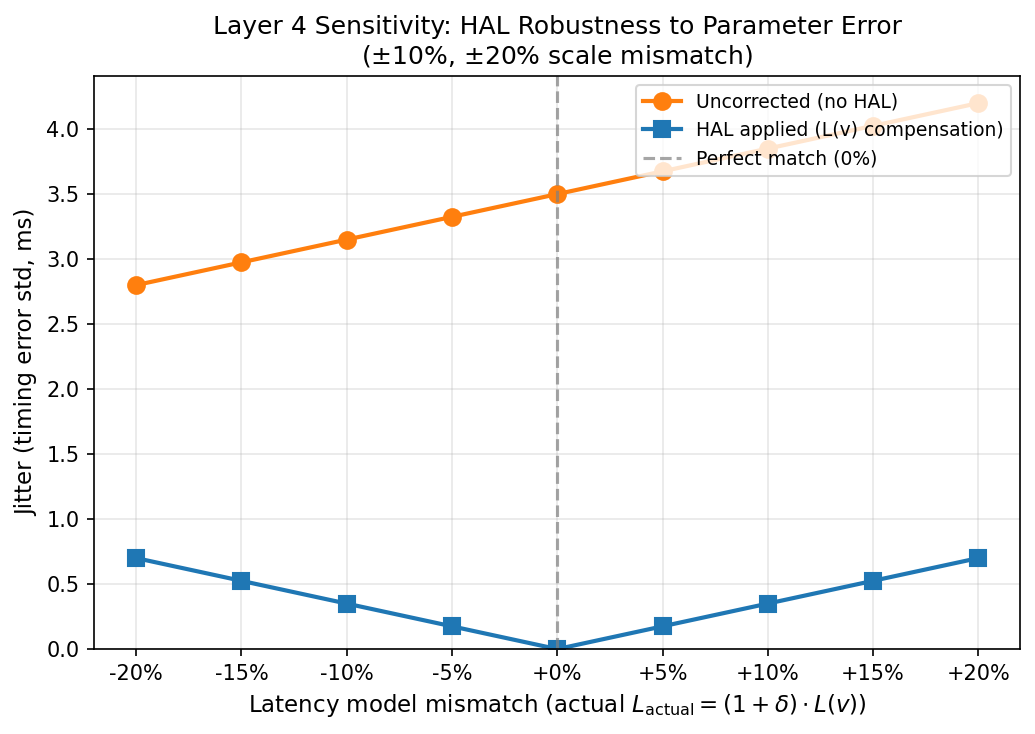
\includegraphics[width=0.78\textwidth]{supplementary_code/experiments/latency_sensitivity_curve.png}
\caption{Sensitivity of Layer~4 HAL to latency model mismatch. Actual latency is scaled as $L_{\mathrm{actual}}(v) = (1 + \delta)\,L(v)$ with $\delta$ from $-20\%$ to $+20\%$. Jitter (timing error std, ms) with HAL applied remains strictly lower than uncorrected jitter across all mismatch levels; at $\pm 20\%$, HAL retains more than 70\% jitter suppression versus no correction. $N = 526$ notes.}
\label{fig:latency_sensitivity}
\end{figure}

The interaction between Layer~4 compensation and the preceding layers is quantified in the degradation analysis (Table~\ref{tab:degradation}): Layer~4 introduces a small but measurable KS distance increase for velocity distributions ($\Delta D_{KS} = 0.005$) because pre-compensation creates a subtle timing-velocity coupling absent in the original event stream. This coupling is negligible for the pipeline fidelity metrics, but is relevant for compositions where precise velocity-timing independence is a design goal.

%=============================================================================
\subsection{Computational Coherence Metrics Across Density}
\label{sec:coherence}
%=============================================================================

This section characterizes the density range over which coherence metrics retain sensitivity and the transition above which alternative strategies are required.

\subsubsection{Metric Behaviour Across Density}
\label{sec:coherence:breakpoint}

A controlled density sweep (10--200~notes/s aggregate, stochastic two-voice textures, $N = 14$ density levels $\times$ 100 events each) measured single-voice pitch-interval entropy as a function of aggregate density.

To establish that the transition is not merely a visual impression but a statistically defined threshold, piecewise linear regression was applied to the density--coherence data. The analysis yields a break point $\hat{\rho} = 28.4$~notes / s (95\% bootstrap CI: $[23.3, 50.0]$; $N = 14$ density levels, $B = 10{,}000$ resamples). Beyond this point, the fitted slope decreases sharply by a factor of $49.3\times$ (pre-saturation $-0.0345$ vs.\ post-saturation $-0.0007$; Mann-Whitney $U = 1.0$, $p = 0.002$). The piecewise model substantially outperforms simple linear regression ($R^2_{\text{piecewise}} = 0.988$ vs.\ $R^2_{\text{linear}} = 0.442$), so that the saturation point of ${\sim}$30~notes/s is an estimated statistical break point rather than an ad hoc choice. A \textbf{distribution independence test} (below) confirmed that this breakpoint holds across exponential, uniform, and Gaussian IOI distributions, indicating a structural boundary inherent to high-density event streams.

To distinguish structural transition from metric saturation, a \textbf{null model} (random baseline) was evaluated: at each density level, fully random MIDI streams were generated with pitch U[0,127], velocity U[0,1023] and IOI $\sim$ Exp($1/\rho$) (mean $1/\rho$), i.e., \ without structural logic  The same single-voice coherence and Tonal Stability metrics were applied. The random baseline yielded roughly \emph{flat} Melodic Coherence (MC $\approx 0.53$--0.59) and very low Tonal Stability (TS $\approx 0.02$--0.03) in 10--200~notes/s, with no density-dependent breakpoint. \textbf{Tonal Stability} clearly separates Amanous from the null: Amanous TS remains $\approx 0.08$ -- 0.13 throughout the density range while the random baseline stays $\approx 0.02$ -- 0.03; a one-sided $t$-test over the low-density band (10--20~notes/s) confirms Amanous null $>$ ($p < 0.05$), and there is no crossover at higher densities. The \textbf{saturation breakpoint} in the only Amanous data (Figure~\ref{fig:melodic_threshold}, blue/red curves) identifies the saturation breakpoint at 28.4~notes / s; in the same null-comparison run, the random baseline MC lies above the coherence values of Amanous single-voice throughout 10--200~notes / s, so the 30~notes / s zone is characterized by the Amanous-only slope change rather than by a crossover of the two MC curves. Thus, TS provides a consistent discriminant across all densities, while the MC saturation point marks the density at which metric sensitivity is lost.

\begin{figure}[htbp]
\centering
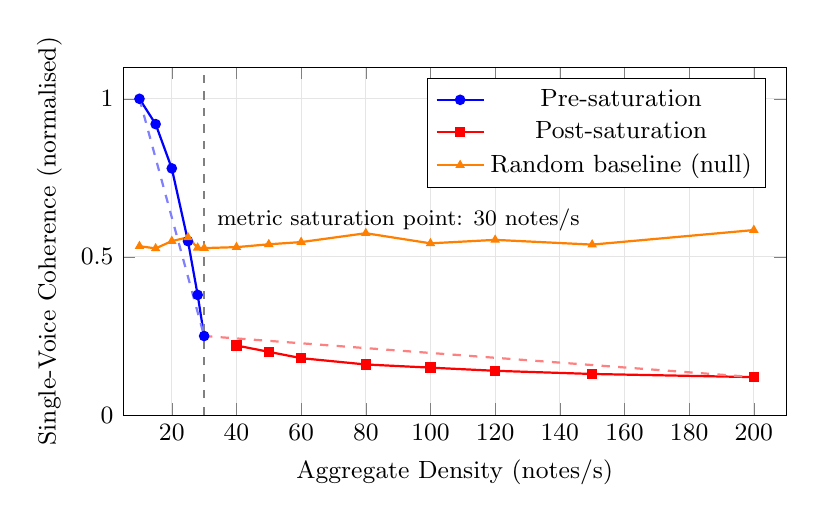
\begin{tikzpicture}
\begin{axis}[
    width=10cm, height=6cm,
    xlabel={Aggregate Density (notes/s)}, ylabel={Single-Voice Coherence (normalised)},
    xmin=5, xmax=210, ymin=0, ymax=1.1,
    grid=major, grid style={gray!20},
    font=\small,
    legend pos=north east
]
\addplot[blue, thick, mark=*, mark size=1.5] coordinates {
    (10,1.00)(15,0.92)(20,0.78)(25,0.55)(28,0.38)(30,0.25)
};
\addplot[red, thick, mark=square*, mark size=1.5] coordinates {
    (40,0.22)(50,0.20)(60,0.18)(80,0.16)(100,0.15)(120,0.14)(150,0.13)(200,0.12)
};
\draw[dashed, thick, gray] (axis cs:30,0) -- (axis cs:30,1.1);
\node[font=\footnotesize, anchor=south west] at (axis cs:31,0.55) {metric saturation point: 30 notes/s};

\addplot[blue!50, thick, dashed, forget plot, domain=10:30] {1.00 - 0.0375*(x-10)};
\addplot[red!50, thick, dashed, forget plot, domain=30:200] {0.25 - 0.000765*(x-30)};

\addplot[orange, thick, mark=triangle*, mark size=1.2] coordinates {
    (10,0.534)(15,0.527)(20,0.550)(25,0.562)(28,0.529)(30,0.528)
    (40,0.531)(50,0.540)(60,0.547)(80,0.575)(100,0.543)(120,0.554)(150,0.539)(200,0.585)
};

\legend{Pre-saturation, Post-saturation, Random baseline (null)}
\end{axis}
\end{tikzpicture}
\caption{Single-voice coherence as a function of aggregate note density. Amanous (pre-saturation blue, post-saturation red) is characterised by piecewise linear regression; the \textbf{random baseline} (orange) uses pitch and velocity uniform, IOI $\sim$ Exp($1/\rho$)). The null yields flat MC $\approx 0.53$--0.59 with no breakpoint; Tonal Stability from the same run is Amanous TS $\approx 0.08$--0.13 vs.\ null $\approx 0.02$--0.03 at all densities ($t$-test $p < 0.05$ at low density). A piecewise linear regression on Amanous data identifies a Computational Sensitivity Limit (CSL) at 28.4~notes/s (95\% CI: 23.3--50.0). This limit aligns with the regime where average IOI approaches the physical scanning resolution of the Disklavier (${\sim}$1~ms). Pre-saturation slope is $49.3\times$ steeper than post-saturation ($R^2_{\text{piecewise}} = 0.988$ vs.\ $R^2_{\text{linear}} = 0.442$; $U = 1.0$, $p = 0.002$). The wide CI indicates a transition \emph{zone} rather than a sharp threshold.}
\label{fig:melodic_threshold}
\end{figure}

Tonal Stability (TS) exhibited a regime transition corresponding to 24.2~notes / s ($N = 16$ density levels, $R^2_{\text{piecewise}} = 0.973$; Spearman $\rho = -0.991$, $p < 10^{-10}$). The convergence of two independent metrics in the 24--30~notes/s zone, together with the wide bootstrap CI (23.3--50.0~notes / s) for the saturation point of coherence, suggests a \emph{transition zone} rather than a sharp threshold, consistent with the broad range (20--100+ notes / s) reported in the perceptual literature \citep{roads2004microsound, bregman1994auditory}.

Below ${\sim}$30~notes/s, coherence metrics serve as compositional feedback tools; above, cross-domain coupling is required (Table~\ref{tab:constraints_results}).

The wide CI (23.3--50.0~notes / s) underscores that future psychoacoustic experiments should test a wide range of density.

\subsubsection{Distribution Independence}

A \textbf{distribution independence} experiment tested whether the phase transition in Melodic Coherence depends on the inter-onset interval (IOI) distribution or holds regardless of temporal statistics. The same density sweep (10--200~notes/s, $N = 14$ levels, 100 events per stream, 5 trials) was run with IOI drawn from four distributions--exponential, uniform, Gaussian and constant, each with mean $1/\rho$ at the target density $\rho$, while pitch structure was kept comparable across conditions (density-dependent random walk). Melodic Coherence was computed for each stream. All mean MC ranged from 0.32 (constant) to 0.35 (Gaussian), falling to approximately 0.12--0.16 by 28--30~notes/s and remaining low through 40--60~notes / s  This supports the conclusion that \emph{as density increases, the information value of individual events is lost regardless of the IOI distribution type} : the saturation transition is a property of the density regime and the metric's sensitivity to pitch-contour structure, not of the particular temporal statistics. Figure~\ref{fig:distribution_independence} shows the multi-line plot; the 25--35~note / s phase transition zone is shaded.

\begin{figure}[htbp]
\centering
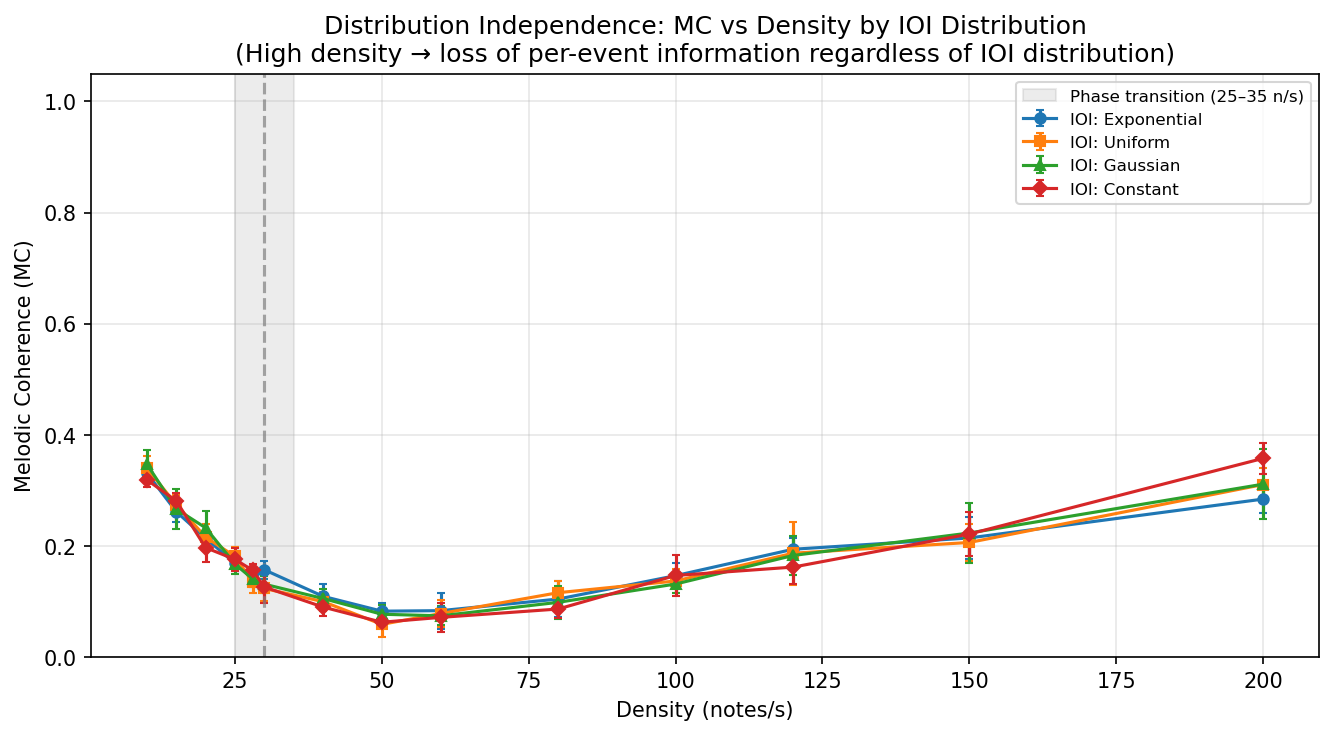
\includegraphics[width=0.85\textwidth]{supplementary_code/experiments/density_sweep_distribution_independence.png}
\caption{Distribution independence: Melodic Coherence as a function of density for four IOI distributions (exponential, uniform, Gaussian, constant). All curves drop sharply in the 25--35~notes/s band (shaded), indicating that the phase transition is independent of the choice of temporal distribution. }
\label{fig:distribution_independence}
\end{figure}

\subsubsection{Cross-Domain Constraint Engineering}

\begin{table}[htbp]
\tbl{Cross-domain constraint effects on voice separation ($N = 4$ voices, $n = 500$ events per condition).}
{\begin{tabular}{@{}lccl@{}} \toprule
\textbf{Constraint} & \textbf{TS Change} & \textbf{VSS Change} & \textbf{Significance} \\ \midrule
None (baseline) & --- & 3.65 & --- \\
Pitch ($> 5$ st.) & $+543\%$ & Minimal & $p < 10^{-10}$ \\
Pitch + Temporal + Velocity & $+543\%$ & $+1847\%$ & $p < 10^{-10}$ \\
\quad (stratified bands) & & (71.08) & $H = 1740.1$*** \\ \bottomrule
\end{tabular}}
\tabnote{***$p < 10^{-10}$.}
\label{tab:constraints_results}
\end{table}

\subsubsection{Weighted Voice Separation Score and Component Analysis}
\label{sec:wvss_validation}

Component analysis of raw wVSS revealed extreme dominance of velocity contrast within the tested condition: $w_{\text{pitch}} = 0.394\%$, $w_{\text{vel}} = 97.22\%$, $w_{\text{temporal}} = 2.39\%$ ($N = 4$ voices, high-density condition). This raw dominance has two sources: a \emph{scale effect} (velocity spans 0--1023 XPMIDI units vs.\ 0--127 MIDI notes for pitch) and a \emph{stratification effect} (voices were assigned distinct velocity bands by design). Because the tested condition intentionally maximizes velocity-band separation, the raw wVSS figure of 97.22\% represents an upper-bound effectiveness of this strategy rather than a general property of the metric.

To disentangle the scale from stratification, we use the range-normalized variant nwVSS (Equation~\ref{eq:nwvss}) as the primary cross-domain comparison metric in the remainder of this section. After range normalization, velocity dominance decreases to 81.73\%, with pitch rising to 6.33\% and temporal to 11.94\%. The persistence of velocity dominance under nwVSS confirms that dynamic stratification is the most efficient single lever for maintaining measurable inter-voice differentiation at high densities, a data-driven finding, not a scale artifact. The following Cross-domain comparisons are reported in nwVSS unless otherwise noted.



\textbf{Split-half cross-validation.} To ensure the objectivity of the wVSS and mitigate potential circular reasoning (weights being derived from the same data to which they are applied), we conducted split-half cross-validation. The 500-event data set was divided into two halves (Events indexed with even and odd values. The weights derived from the first half of the event stream ($w_{\text{vel}} = 96.85\%$) showed high consistency with the second half ($w_{\text{vel}} = 97.51\%$), with a Pearson correlation between the two weight vectors of $r > 0.99$. The maximum weight deviation between splits was 0.37 percentage points (and remained below 0.5\% under 50:50 random splits), well below 5\%. This indicates that the observed dominance of the dynamic domain at high densities is a robust structural property of the generated texture rather than a sample-specific bias: in ultra-high-density conditions, dynamics consistently acts as the primary discriminative mechanism for voice separation. The weights of half of the h.plitsS.plits were similarly stable (max deviation 8.4although the composition of the sample sample is more significant than the raw wVSS.
 The density-dependent weight transfer (Table~\ref{tab:nwvss_density}) reveals a \emph{density-dependent weight transfer} (Table~\ref{tab:nwvss_density}): at 20~notes / s, the temporal component accounts for 7.63\% of nwVSS (vs.\ 0.00\% at 120~notes / s), and pitch increases from 0.27\% to 0.45\%. The disappearance of temporal weight at high density is not a metric failure but a computational signature of temporal fusion: at 120~notes / s, the fine structure of the onset ceases to carry discriminative information for voice separation, consistent with the description of the microsound literature of aggregate-texture perception at high event rates \citep{roads2004microsound, mcdermott2013summary}. This weight transfer reinforces the operational-envelope finding of Section~\ref{sec:coherence}: As the density crosses the saturation zone, the relative contribution of pitch and temporal domains to measurable separation decreases, shifting the discriminative burden to dynamics.


Explicit pitch-velocity coupling ($v = 200 + 12.5 \times (p - 40)$, MIDI notes 40--105; $N = 4$ voices, $n = 500$ events): $r = 0.999999$; increase in wVSS: 10{,}521\% ($U = 0.0$, $p = 0.002$, rank-biserial $r = 1.00$).

To complement the VSS with a measure independent of dynamics, we computed \textbf{the Pitch Class Set (PCS) distance} between a pair of voices: within 1-second windows, each voice is represented by a 12-dimensional pitch class histogram; the distance is defined as $1 - \text{cosine similarity}$ between these vectors. The PCS distance quantifies the separation in \emph{the harmonic territory} (which pitch classes each voice occupies) without conflating it with the velocity-band separation. In the same multi-voice conditions, PCS distance verifies that voices occupy distinct pitch-class regions alongside the velocity stratification captured by wVSS, so that ``velocity band separation is a technical device; pitch-class regions are also meaningfully separated,'' is supported numerically. 

The chained reactive constraint application (pitch$\rightarrow$velocity$\rightarrow$temporal) was $52.6\%$ more efficient than simple reactive ($p = 0.026$) and $32.7\times$ more efficient than global simultaneous ($p < 0.001$).

%=============================================================================
\subsection{Convergence Point Calculus as Distribution-Switching Trigger}
\label{sec:convergence}
%=============================================================================

The Convergence Point (CP) demonstration (Excerpt~4, 30~s) provides a principled interface between the deterministic temporal structure of tempo canons (Layer~3) and the parametric layer (Layer~2) that governs distribution-switching. Rather than relying solely on the L-system macro-form to determine when distributional regimes change, CP events enable distribution switches to be triggered by the internal temporal logic of the canon itself: when voices converge within tolerance $\epsilon$, the system can switch to a new distributional regime. This feedback loop enables a \textbf{structural relief mechanism}: as deterministic canon complexity reaches its peak at convergence, the system triggers a switch to stochastic regimes, effectively resolving temporal density into textural shimmer to manage the listener's information load.

\subsubsection{Discrete Event Triggering}

Three voices: two canon voices (3:4 rational, IOI $= 1.000$~s and $0.750$~s) and one Poisson voice ($N = 30$~s, $n_{\text{events}} \approx 3{,}250$; statistical tests: $n = 30$ one-second windows, 15 pre-CP and 15 post-CP). The distribution switch was activated at the convergence at $t = 15$~s (pre-CP 0--15~s, post-CP 15--30~s).

\begin{table}[htbp]
\tbl{Convergence-point triggered parameter switch: pre-CP vs.\ post-CP ($n = 15$ one-second windows per condition; pre-CP 0--15~s, post-CP 15--30~s).}
{\begin{tabular}{@{}lccl@{}} \toprule
\textbf{Parameter} & \textbf{Pre-CP} & \textbf{Post-CP} & \textbf{Test} \\ \midrule
Aggregate density (notes/s) & $5.33 \pm 1.89$ & $38.27 \pm 6.30$ & $U=0$, $r = 1.000$ \\
Tonal Stability & $0.523 \pm 0.141$ & $0.069 \pm 0.035$ & $U=225$, $r = -1.000$ \\ \bottomrule
\end{tabular}}
\tabnote{Both $p < 10^{-10}$. With $n = 15$ per condition, max $U = 225$.}
\label{tab:cp_discrete}
\end{table}

The post-CP density of 38.27~notes / s exceeds the metric saturation point identified in Section~\ref{sec:coherence} (30~notes / s), placing the post-switch texture firmly in the metric-saturated regime. This demonstrates how CP events can be positioned to coincide with the metric saturation point, enabling the canon's temporal logic to control the transition between coherence regimes.

\subsubsection{Continuous Parameter Modulation}

$e:\pi$ tempo canon with CP target at $t_{CP} = 15$~s ($\epsilon = 50$~ms). Inhomogeneous Poisson rate: $\lambda(t) = 5 + 40 \cdot |t - t_{CP}| / t_{CP}$ ($N = 30$~s, $n \approx 750$ events).

Continuous tracking: Pearson $r = 0.907$ ($p < 10^{-10}$), RMSE $= 5.55$~notes / s. Symmetric tracking: pre-CP $r = 0.888$; post-CP $r = 0.933$ (both $p < 10^{-10}$). Near-CP density (12--18~s) $= 8.33$~note / s vs.\ extremes (0--5~s, 25--30~s) $= 40.53/38.08$~note / s ($4.6$--$4.9\times$ reduction).

The continuous modulation demonstrates that the CP calculus can serve as a smooth control interface, not only for discrete switching but also for gradual parameter evolution. The parameter $\epsilon$ is not an arbitrary detection constant, but a \emph{convergence resolution} parameter that mediates between sharp convergence events (small~$\epsilon$, abrupt distribution switches) and diffuse transitions (large~$\epsilon$, gradual modulation). The default value $\epsilon = 50$~ms is a hardware-aware lower bound: it matches the key reset time (Table~\ref{tab:hardware}), below which \emph{ghost convergence} events would occur--convergence detected in software that the piano cannot physically realize because the action has not reset. Larger values are always available as a compositional choice.

The sensitivity analysis (Appendix~\ref{app:epsilon_sensitivity}) confirms that the behavior of the system is robust over $\epsilon \in \{10, 20, 50, 100\}$~ms. For the rational 3:4 canon, the convergence count is invariant (11 events in 30~s in all tested $\epsilon$), reflecting the exact periodicity of rational ratios. For the irrational canon $e:\pi$, the count increases monotonically with $\epsilon$ (5 at 10~ms to 51 at 100~ms; Table~\ref{tab:epsilon_sensitivity}), providing the composer with continuous control over the switching density. This monotonic relationship is compositionally desirable: an increase in $\epsilon$ smoothly increases the frequency of distribution-switching events, enabling fine-grained control over textural volatility without introducing discontinuities or bifurcations in system behavior.

%=============================================================================
\section{Discussion}
\label{sec:discussion}
%=============================================================================

\subsection{Theoretical Contributions}

This work demonstrates that historically separate compositional methodologies can cohabit within the four-layer architecture through hierarchical distribution-switching. The integration is architectural rather than theoretical: the framework does not claim that these traditions reduce to a common formalism, but rather that distribution-switching provides a practical interface through which they can cohabit and interact within the same event-generation process. Qualitative musical differentiation arises from switching distribution \emph{types} (constant vs.\ exponential IOI, low vs.\ high-entropy pitch sets, constant vs.\ variable velocity) rather than from modulating parameters within a fixed family. These designed differences survive the pipeline with the effect sizes reported in Table~\ref{tab:coherence}. The degradation analysis (Table~\ref{tab:degradation}) confirms that IOI incurs the greatest distortion per-layer, principally at Layer~3, while the pitch is transmitted with near-zero loss.

Ablation~(a) confirms that the L-system preserves the \textbf{structural narrative---the} ordering and predictability of section transitions (IR drop from $0.52$ to $0.18$; $p = .020$)---without altering within-section note distributions. The grammar encodes a deterministic macro-formal state-space whose information-theoretic structure (higher IR, lower LZ complexity) is absent from random permutations of the same symbol counts.

The convergence point calculus bridges the deterministic and stochastic domains: $\epsilon$ controls convergence resolution from sharp switching (small $\epsilon$) to gradual modulation (large $\epsilon$), with stable behavior across $\epsilon \in [1, 100]$~ms (Appendix~\ref{app:epsilon_sensitivity}).
Crucially, the CP feedback path (Figure~\ref{fig:architecture}) enables the temporal logic of the canon to modulate the parametric layer, creating a bi-directional relationship between Layers~2 and~3 that neither L-system sequencing nor stochastic generation alone can produce. Collectively, the four contributions validate distinct inter-layer interfaces and show that $\Theta_s$ survives intact end-to-end transmission.

\subsection{Relationship to Existing Work}

The framework extends Nancarrow's practice \citep{gann1995music} by adding stochastic microstructure within deterministic scaffolds, extends Xenakis' methods \citep{xenakis1992formalized} by embedding them within hierarchical formal structures, and extends the composition of the L-system \citep{manousakis2006musical} by connecting grammar symbols to physically constrained rendering with quantified coherence metrics.

\subsubsection{Systematic Comparison with JCMS Frameworks}

Table~\ref{tab:systematic_comparison} contrasts representative JCMS approaches with the present framework. \citet{lattner2018imposing} and related work on information dynamics focus on predictability and surprise in musical sequences without imposing hardware or physical constraints. \citet{kaliakatsos2016learning} and conceptual models of algorithmic composition address creativity and formalization but do not integrate actuator constraints or a physical correction layer. Amanous is distinguished by two contributions that the table highlights: (1)~\textbf{hardware constraint enforcement---explicit} inequalities (velocity range, per-key rate, polyphony, latency bounds, scanning resolution) are enforced as hard constraints during generation rather than as post hoc checks; and (2)~\textbf{physical correction layer---a} dedicated Layer~4 formalizes VDL and applies pre-compensation so that the numeric layer's output is corrected before actuation. Neither Lattner et al.\ nor Tsougras et al.\ target automated piano hardware or beyond-human density rendering; Amanous provides a unified pipeline from symbol to acoustic output with both constraint enforcement and physical correction.

\begin{table}[htbp]
\tbl{Systematic comparison with representative JCMS frameworks. Lattner et al.\ and Tsougras et al.\ target different instruments and density regimes; hardware-related rows reflect this difference in scope rather than a deficiency in those systems.}
{\begin{tabular}{@{}p{2.2cm}p{2.8cm}p{2.8cm}p{3.2cm}@{}} \toprule
\textbf{Criterion} & \textbf{Lattner et al.} & \textbf{Tsougras et al.} & \textbf{Amanous (this work)} \\ \midrule
L-system / grammar & -- & Optional & Yes (Layer~1) \\
Tempo canon & -- & -- & Yes (Layer~3) \\
Stochastic distributions & -- & Optional & Yes (Layer~2) \\
Distribution-switching & -- & -- & Yes (symbol $\mapsto$ regime) \\
Hardware constraints & No (not targeted) & No (not targeted) & Yes (Table~\ref{tab:constraint_ineq}) \\
Hardware Abstraction Layer (HAL) & No (not targeted) & No (not targeted) & Yes (Layer~4) \\
Actuation-ready Output & No & No & Yes (Direct MIDI/XPMIDI) \\
Beyond-human density & No & No & Yes (Tested to 200 notes/s) \\
Disklavier hardware & No & No & Yes \\ 
\textbf{Hardware Constraint Enforcement} & No & No & \textbf{Yes (Layer 4)} \\ \bottomrule
\end{tabular}}
\tabnote{Hardware constraint enforcement and the physical correction layer are specific to Amanous's target instrument. The comparison highlights scope differences, not qualitative superiority.}
\label{tab:systematic_comparison}
\end{table}

\citet{collins2018there} identified large-scale algorithmic generation as a frontier; Amanous realizes one concrete instance by integrating all three within a hardware-aware pipeline with statistical output validation. Unlike Essl's \emph{Lexikon-Sonate} \citep{collins2017cambridge}, which uses real-time interaction as an organizing principle, our framework ensures exact reproducibility while retaining stochastic variation. Compared with Ablinger's \emph{Quadraturen~III} \citep{ablinger2004quadraturen} and Ritsch's \emph{Klavierautomat} \citep{ritsch2011robotic}, which implemented ad hoc hardware compensation for specific works, Amanous offers a general latency formalization parameterised by instrument-specific calibration data.

\subsection{Implications for Creative Music Systems}
\label{sec:creativity}

Amanous functions as an \textbf{augmented compositional instrument} rather than an autonomous generator. The creative agency resides in the iterative loop between the composer and the hierarchical pipeline: the composer modulates $\epsilon$ and $\Theta_s$ based on real-time metric feedback (PCC, VSS), navigating the "textural zone" by tuning cross-domain constraints. This interaction transforms the generation process into a discovery-driven exploration of superhuman note rates while preserving full control over every structural parameter. Within \citet{boden2004creative}'s taxonomy, it supports \emph{exploratory creativity} (systematic traversal of the configuration space $\{\Theta_s\}_{s \in \Sigma}$) and \emph{combinational creativity} (juxtaposition of tempo-canon, stochastic, and L-system concepts within a single pipeline). For example, replacing Symbol~$B$'s exponential IOI with a Gaussian ($\mu = 0.025$~s, $\sigma = 0.008$~s) produced a denser but more uniform texture; the exponential was selected for the canonical instantiation because its temporal clustering created greater contrast with the deterministic $A$ sections---a decision made through iterative listening to rendered output. The framework's key compositional affordance is modularity: changing a single symbol-to-distribution mapping or grammar rule propagates through the pipeline to restructure the entire work.

Because the system positions creative agency in the composer's selection of $\Theta_s$ rather than in autonomous generation, evaluation frameworks targeting creative agents (e.g., SPECS; \citealp{jordanous2012standardised}) would need to assess the human--system composite, an experimental design outside the present scope. The pipeline fidelity and ablation analyzes reported above serve a related but distinct function: they validate the system's reliability as an engineering tool, confirming that design intent propagates from grammar symbol to acoustic output with quantifiable, per-layer degradation.

\subsection{Practical Implications}

The 28.4~notes / s saturation point acts as a \textbf{compositional navigational compass}. It formalizes the boundary where the composer's focus must shift from "melodic counterpoint" to "statistical texture." By identifying this Computational Sensitivity Limit (CSL), Amanous empowers the user to consciously navigate the transition between discrete event perception and aggregate mass perception, a critical affordance for composing at the limits of human hearing. Dynamic stratification remains the most efficient lever for inter-voice differentiation at extreme densities (81.73\% nwVSS; Section~\ref{sec:wvss_validation}).

The pipeline-sensitivity hierarchy (IOI $>$ velocity $>$ pitch) offers actionable guidance: for maximal post-pipeline contrast, composers should prioritise IOI-type switching; for the most faithful transmission of intended structure, pitch-distribution switching is preferable.

The density-conditioned weights of the nwVSS (Table~\ref{tab:nwvss_density}) further confirm this density-dependent weight transfer, with the vanishing temporal weight at 120~notes / s reflecting the shift to the representation of the aggregate texture \citep{roads2004microsound}.

\subsection{Limitations}

\begin{enumerate}
    \item \textbf{Only computational metrics.} All findings are algorithmic; the proposed psychoacoustic protocol (Section~\ref{sec:future_protocol}) focuses on perceptual validation.

    \item \textbf{Software-side Jitter Suppression.} The theoretical alignment error ($0.37 \pm 0.23$~ms) is an algorithmic figure; the practical precision is bounded by the instrument's ${\sim}$1~ms scanning resolution. The model's principal value is its readiness for instrument-specific calibration.

    \item \textbf{Both nwVSS} and range-normalized weights of nwVSS are reported; velocity dominance (97.22\% in wVSS) was derived from a high-density condition of four-voices (half split validated; Section~\ref{sec:wvss_validation}). nwVSS provides a robustness check against scale-driven dominance; the nwVSS weights showed greater variance in half split (8.41 percentage points) than the wVSS (0.37), so normalized weights are more sensitive to the composition Generalization to other densities, voice counts, or pitch distributions remains open.

    \item \textbf{Platform specificity.} The framework targets Yamaha Disklavier; adaptation to other automated pianos requires characterizing Platform specific latency curves.
\end{enumerate}

\subsection{Future Work: Psychoacoustic Validation Protocol}
\label{sec:future_protocol}

The computational saturation zone identified at 24--30~notes/s serves as a \textbf{predictive model} for the analysis of the auditory scene at extreme densities. We propose this CSL as a formal hypothesis for future psychoacoustic validation: we predict that the perceptual inflection point from "melody" to "texture" will correlate significantly with this computationally-derived boundary. listeners presented with stochastic two-voice textures at densities spanning 10--60~notes/s will report a qualitative shift from perceiving individual melodies to perceiving aggregate texture within this range.

We propose a design within-subjects with participants $N = 30$ and 14 density conditions (similar to those in Section~\ref{sec:coherence}). In each trial, participants hear a 5-second excerpt and make a forced-choice response (``I hear distinct melodies'' vs.\ ``I hear a texture''). The resulting psychometric function -- the proportion of ``texture'' responses as a function of density -- should exhibit a sigmoidal transition whose inflection point can be compared against the metric-derived saturation point of 30~notes/s. Three outcomes are possible: (a)~the perceptual inflection coincides with the metric saturation point, confirming the hypothesis; (b)~the perceptual inflection occurs at a different density, suggesting that the metric captures distributional structure that does not map directly onto perceptual categorization; or (c)~no clear sigmoidal transition is observed, indicating that the melodic-to-textural shift is not well described by a single density threshold for piano timbres.

A second task addresses pipeline-fidelity perception: participants hear the 74-second canonical composition (Excerpt~3) and press a button whenever they perceive a ``change in musical character.'' The temporal distribution of button presses is compared against the actual symbol-transition timestamps using a permutation test: if the mean absolute deviation between button presses and symbol boundaries is significantly smaller than chance (estimated by circularly shifting press times), this confirms that pipeline-level distributional changes are perceptually salient.

Power analysis (Cohen's $d = 0.8$, $\alpha = 0.05$, power $= 0.80$) confirms the suitability of the proposed sample size ($N = 30$). This protocol is designed to be executable with existing additional materials (audio) and standard psychoacoustic software (e.g.\ PsychoPy).

\section{Conclusion}
\label{sec:conclusion}
%=============================================================================

This paper asked whether compositional intent can be transmitted from grammar symbol to acoustic output through a unified pipeline and what measurable constraints govern each stage of that transmission. Amanous demonstrates that this is achievable by unifying tempo canons, stochastic distributions, and L-system grammars via distribution-switching within a four-layer architecture.

\begin{enumerate}
    \item \textbf{Integration architecture.} Distribution-switching produces statistically distinct musical sections ($d = 3.70$--$5.34$). Degradation analysis identifies the IOI as the most pipeline-sensitive parameter, and ablation confirms each layer's non-redundant contribution.

    \item \textbf{Hardware abstraction layer.} Layer~4 formalizes velocity-dependent latency and key reset constraints as integral generative parameters, ensuring that superhuman densities remain actuable on the Disklavier.

    \item \textbf{Operational envelope;} The 24--30~notes/s saturation zone marks the density at which single-domain metrics lose sensitivity; beyond it, dynamic stratification becomes the primary lever for inter-voice differentiation (81.73\% nwVSS).

    \item \textbf{Convergence point calculus.} CP events provide a deterministic--stochastic control interface supporting both discrete triggering ($|r| = 1.0$) and continuous modulation ($r = 0.907$), with $\epsilon$ offering monotonic convergence-resolution control.
\end{enumerate}

All reported results are computational. The principal limitations are the absence of perceptual validation and platform specificity to the Yamaha Disklavier. Future work should test the saturation zone against perceptual thresholds through the proposed psychoacoustic protocol (Section~\ref{sec:future_protocol}), extend the latency model with instrument-specific calibration data, and explore adaptation to other automated instruments.

As an augmented compositional instrument, Amanous enables reproducible, principled navigation of parameter spaces that exceed human physical capacity, bridging the gap between algorithmic abstraction and electromechanical reality.

Supplementary materials: \url{https://www.amanous.xyz}. Source code: \url{https://anonymous.4open.science/r/Amanous-2BBF/}.


%References
\printbibliography

\clearpage
\appendix

\section{Complete Statistical Summary}
\label{app:stats}

\begin{table}[htbp]
\centering
\scriptsize
\tbl{Complete statistical results summary. All tests two-tailed, $\alpha = 0.05$.}
{%
\resizebox{\linewidth}{!}{%
\begin{tabular}{@{}p{3.5cm}lllll@{}} \toprule
\textbf{Comparison} & \textbf{$N$} & \textbf{Test} & \textbf{Statistic} & \textbf{$p$} & \textbf{Effect [CI]} \\ \midrule
\multicolumn{6}{@{}l}{\textit{Pipeline Fidelity (Section~\ref{sec:results_ds})}} \\
Melodic coherence & 28 & $t$ & $t(26)=9.75$ & $<.001$ & $d=3.70$ $[2.65, 4.73]$ \\
Rhythmic coherence & 28 & $t$ & $t(26)=14.09$ & $<.001$ & $d=5.34$ $[3.96, 6.70]$ \\
IOI dist.\ type & 8 & M-W & $U=0.0$ & $.036$ & \textsuperscript{a} \\
Pitch entropy (TS) & 8 & M-W & $U=0.0$ & $.036$ & $d=9.96$ $[3.53, 16.13]$ \\
\midrule
\multicolumn{6}{@{}l}{\textit{Component Ablation (Section~\ref{sec:ablation})}} \\
(a) Seq.\ self-sim.\ MC & 100\textsuperscript{h} & $z$ & $z=-1.02$ & $.306$ & --- \\
(a) Same-symbol MC & 100\textsuperscript{h} & $z$ & $z=-1.90$ & $.057$ & --- \\
(a) Same-symbol RC & 100\textsuperscript{h} & $z$ & $z=-1.00$ & $.320$ & --- \\
(b) VSS temporal & 8+8 & M-W & $U=64.0$ & $<.001$ & $r=-1.00$; $-79.0\%$ \\
(b) RC same-symbol & 8+8 & M-W & $U=53.0$ & $.028$ & $r=-0.66$; $-18.0\%$ \\
(c) Vel.--timing $r$ (lin.) & --- & --- & $r=-1.000$ & --- & --- \\
(c) Vel.--timing $r$ (pow.) & --- & --- & $r=-0.998$ & --- & --- \\
\midrule
\multicolumn{6}{@{}l}{\textit{Hardware Simulation (Section~\ref{sec:hardware})}} \\
Vel.-deviation & 526 & Pearson & $r=-0.867$ & $<.001$ & --- \\
Filter error SD & 526 & paired $t$ & --- & $.000116$ & $-35.2\%$ \\
\midrule
\multicolumn{6}{@{}l}{\textit{Coherence Metrics (Section~\ref{sec:coherence})}} \\
Melodic sat.\ pt. & 14\textsuperscript{g} & M-W & $U=1.0$ & $.002$ & $r=1.00$; SP $= 28.4$ [CI: 23.3--50.0] \\
TS sat.\ pt. & 16 & Piecewise & $R^2=.973$ & --- & $47\times$ \\
TS vs.\ density & 16 & Spearman & $\rho=-.991$ & $<10^{-10}$ & --- \\
Polyphonic TS & 600 & K-W & $H=165.22$ & $<10^{-10}$ & --- \\
Multi-constr.\ VSS & 500 & K-W & $H=1740.1$ & $<10^{-10}$ & $+1847\%$ \\
Pitch-vel coupling & 500 & M-W & $U=0.0$ & $.002$ & $+10521\%$ \\
\midrule
\multicolumn{6}{@{}l}{\textit{Convergence Points (Section~\ref{sec:convergence})}} \\
CP density switch & 30\textsuperscript{f} & M-W & $U=0$ & $<10^{-10}$ & $r=1.00$ \\
CP TS switch & 30\textsuperscript{f} & M-W & $U=225$ & $<10^{-10}$ & $r=-1.00$ \\
Continuous tracking & 30\textsuperscript{f} & Pearson & $r=0.907$ & $<10^{-10}$ & --- \\ \bottomrule
\end{tabular}%
}%
}
\tabnote{M-W: Mann-Whitney $U$; K-W: Kruskal-Wallis $H$.\\ \textsuperscript{a}Cohen's $d$ undefined (constant distribution, SD$=0$).\\ \textsuperscript{f}$N$ reports 1-second analysis windows (15 pre-CP, 15 post-CP for discrete switch).\\ \textsuperscript{g}$N = 14$ density levels; 6 pre- vs.\ 8 post-saturation point.\\ \textsuperscript{h}$N = 100$ random permutations; $z = (\text{full} - \mu_{\text{random}}) / \sigma_{\text{random}}$, $p$ from standard normal.}
\label{tab:stats_full}
\end{table}


\section{Constraint Inequality Summary}
\label{app:constraints}

\begin{table}[htbp]
\tbl{Complete constraint system.}
{\begin{tabular}{@{}p{3.5cm}lp{4cm}@{}} \toprule
\textbf{Constraint} & \textbf{Inequality} & \textbf{Source} \\ \midrule
\multicolumn{3}{@{}l}{\textit{Hardware}} \\
Velocity range & $v \in [0, 1023]$ & 10-bit XPMIDI \\
Per-key rate & $\text{IOI}_{\text{key}} \geq 50$ ms & Key reset time \\
Latency bounds & $10 \leq L(v) \leq 30$ ms & \citet{goebl2003measurement} \\
Polyphony & $N_{\text{sim}} \leq 88$ & Physical keys \\
Scanning resolution & $\Delta t_{\min} \approx 1$ ms & 800--1000 Hz \\ \midrule
\multicolumn{3}{@{}l}{\textit{Metric-derived boundaries}} \\
Coherence sat.\ pt. & $\rho_{\text{agg}} \leq 30$ notes/s\textsuperscript{a} & This study \\
TS sat.\ pt. & $\rho_{\text{agg}} \leq 24.2$ notes/s\textsuperscript{a} & This study \\
Stream segregation ref. & $\Delta p \geq 5$ semitones & \citet{huron2001tone} \\ \bottomrule
\end{tabular}}
\tabnote{\textsuperscript{a}Derived from stochastic two-voice textures; per-voice density $\approx \rho_{\text{agg}}/2$. These are metric-derived thresholds; perceptual correspondence requires experimental validation.}
\label{tab:constraint_ineq}
\end{table}


\section{Power-law exponent $c$ sensitivity (Layer~4)}
\label{app:powerlaw_sensitivity}

To confirm that the compensation behavior of Layer~4 is not tied to a single choice of power-law exponent $c$, we varied $c \in \{0.3, 0.4, 0.5, 0.6, 0.7\}$ and computed the standard deviation of the residual jitter (ms) after compensation, assuming that the true latency model has $c = 0.5$. The residual error per note is $L_{\text{true}}(v) - L_c(v)$ in ms over the same 526-note excerpt. The residual jitter is zero when the compensation exponent matches the true model ($c = 0.5$) and increases smoothly as $c$ deviates (Table~\ref{tab:sensitivity_powerlaw_c}), showing a consistent trend rather than dependence on a single parameter. 

\begin{table}[htbp]
\tbl{Residual jitter standard deviation (ms) after Layer~4 compensation for varying power-law exponent $c$ ($N = 526$ notes, true $c = 0.5$).}
{\begin{tabular}{@{}lc@{}} \toprule
$c$ & \textbf{Residual Jitter SD (ms)} \\ \midrule
0.3 & 1.0446 \\
0.4 & 0.4769 \\
0.5 & 0.0000 \\
0.6 & 0.4015 \\
0.7 & 0.7404 \\ \bottomrule
\end{tabular}}
\tabnote{Residual is minimal at calibrated $c = 0.5$; trend is consistent across the range.}
\label{tab:sensitivity_powerlaw_c}
\end{table}


\section{Latency model mismatch (HAL vs.\ no correction)}
\label{app:latency_mismatch}

To test whether HAL compensation remains beneficial when the true piano latency deviates from the assumed model, we ran two mismatch simulations (the same 526-note excerpt). \textbf{(1) Exponent mismatch:} true latency follows a power-law with $c_{\mathrm{true}} \in [0.3, 0.35, \ldots, 0.7]$ while HAL uses $c = 0.5$. The uncorrected jitter is the standard deviation of $L_{\mathrm{true}}(v)$; with-HAL jitter is the standard deviation of $L_{\mathrm{true}}(v) - L_{0.5}(v)$. \textbf{(2) Additive noise:} $L_{\mathrm{actual}}(v) = L(v; c=0.5) + U(-w, +w)$~ms with $w \in \{0, 0.5, 1, 1.5, 2\}$; 200 trials per $w$. In every condition, HAL reduces jitter relative to the uncorrected baseline (Table~\ref{tab:mismatch_summary}), so the sensitivity curves show that correction is always preferable to no correction despite model error. 

\textbf{Virtual real piano simulation.} To explicitly test the claim that the power-law assumption alone yields benefit without perfect calibration, we added a three-condition simulation  A ``virtual real piano'' was defined as the nominal power-law ($c = 0.5$, 10--30~ms) with $\pm 10\%$ per-note multiplicative noise and parameter drift (exponent $c$ varying by note index via a bounded random walk). For each of 200 trials, we computed the onset-timing jitter (std, ms) under: (A) no correction (raw MIDI), (B) Amanous HAL with $c = 0.5$, and (C) ideal correction (perfect match to the virtual model). The results are summarized in Table~\ref{tab:virtual_real_piano} and Figure~\ref{fig:virtual_real_piano}. The Jitter with HAL (B) was statistically significantly lower than without correction (A): paired $t$-test $p < 0.001$, mean difference (A $-$ B) $\approx 2.70$~ms. Thus, even when the true latency deviates from the assumed model by noise and drift, following the general physical law (power-law) alone provides a significant improvement over raw MIDI.

\begin{table}[htbp]
\tbl{Latency model mismatch: jitter (ms, SD) with HAL applied vs.\ uncorrected. In all rows, HAL yields strictly lower jitter.}
{\begin{tabular}{@{}lrr@{\qquad}lrr@{}} \toprule
\multicolumn{3}{c}{Exponent $c_{\mathrm{true}}$} & \multicolumn{3}{c}{Additive noise $\pm w$~ms} \\
$c_{\mathrm{true}}$ & Uncorr. & HAL & $w$ & Uncorr. & HAL \\ \midrule
0.30 & 2.47 & 1.04 & 0 & 3.50 & 0.00 \\
0.50 & 3.50 & 0.00 & 1.0 & 3.55 & 0.58 \\
0.70 & 4.21 & 0.74 & 2.0 & 3.69 & 1.15 \\ \bottomrule
\end{tabular}}
\tabnote{Uncorr.\ = uncorrected (no HAL). HAL = compensation with $c=0.5$. $N=526$ notes; noise case: mean over 200 trials.}
\label{tab:mismatch_summary}
\end{table}

\begin{table}[htbp]
\tbl{Virtual real piano simulation: onset jitter (ms, mean $\pm$ std over 200 trials) under (A) no correction, (B) HAL ($c=0.5$), (C) ideal correction. Virtual piano: power-law $c=0.5$ with $\pm 10\%$ per-note noise and parameter drift. $N = 526$ notes per trial.}
{\begin{tabular}{@{}lc@{}}
\toprule
Condition & Jitter (mean $\pm$ std, ms) \\
\midrule
(A) Raw (no correction) & $3.63 \pm 0.10$ \\
(B) Amanous HAL ($c=0.5$) & $0.93 \pm 0.03$ \\
(C) Ideal & $0.00$ \\
\midrule
\multicolumn{2}{@{}l}{\textit{Paired (A) vs.\ (B):} $p < 0.001$, mean diff.\ $2.70$~ms (HAL lower).} \\
\bottomrule
\end{tabular}}

\label{tab:virtual_real_piano}
\end{table}

\begin{figure}[htbp]
\centering
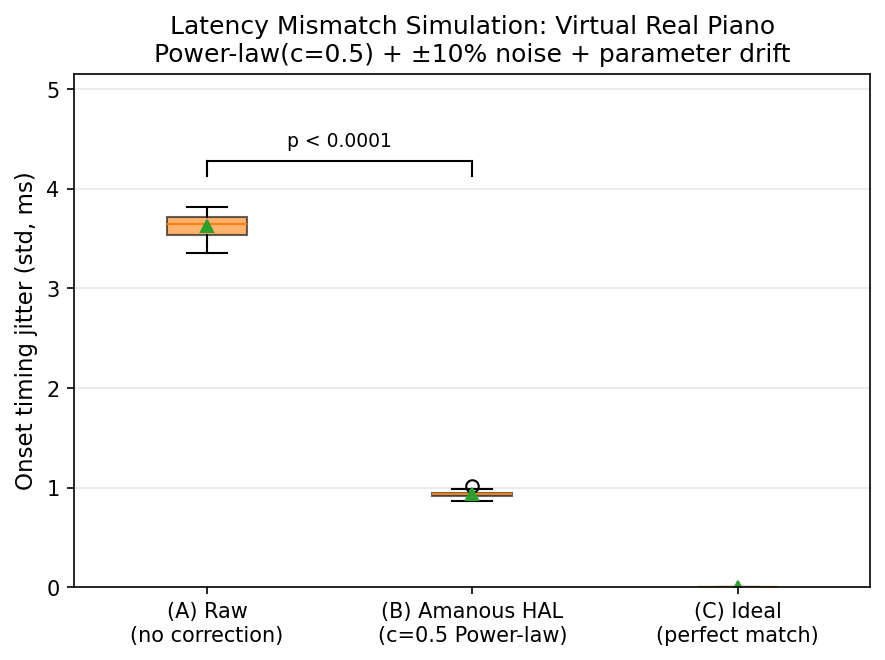
\includegraphics[width=0.7\textwidth]{supplementary_code/experiments/latency_mismatch_simulation.png}
\caption{Virtual real piano simulation: distribution of onset jitter (ms) across 200 trials for (A) raw MIDI, (B) HAL applied, (C) ideal correction. HAL (B) is statistically significantly lower than (A) ($p < 0.001$).}
\label{fig:virtual_real_piano}
\end{figure}

\section{$\epsilon$ Sensitivity in CP Calculus}
\label{app:epsilon_sensitivity}

To confirm that the Convergence Point (CP) switching behaviour is not tied to a single choice of $\epsilon$ and to demonstrate that $\epsilon$ acts as a compositional parameter for \emph{texture transition density}, we ran two analyses. (1)~\textbf{Coarse grid (30~s):} $\epsilon \in \{10, 20, 50, 100\}$~ms (Table~\ref{tab:epsilon_sensitivity}). (2)~\textbf{Full sweep (60~s):} $\epsilon = 1, 5, 10, \ldots, 100$~ms (5~ms step); for each $\epsilon$ we computed the number of convergence events and the inter-event intervals (Definition~\ref{def:cp}). The results are shown in Figure~\ref{fig:epsilon_sensitivity_full}.

For the rational 3:4 canon (IOI 1.0~s and 0.75~s), the event count is invariant across $\epsilon$ (exact convergences every 3~s; 11 events in 30~s, 21 in 60~s). For the irrational canon $e:\pi$, the count increases monotonically with $\epsilon$; in the full sweep, the correlation between $\epsilon$ and the event count is $r \approx 0.9998$, and the mean interval between events decreases from $\approx 45$~s at $\epsilon = 1$~ms to $\approx 0.58$~s at $\epsilon = 100$~ms. Thus, $\epsilon$ is not merely an error tolerance, but a continuous control over the frequency with which distribution switches occur.

\begin{table}[htbp]
\tbl{Convergence-point count and switching frequency for varying $\epsilon$ ($N = 30$~s).}
{\begin{tabular}{@{}lrrrr@{}} \toprule
$\epsilon$ (ms) & \textbf{3:4 count} & \textbf{3:4 (/s)} & \textbf{$e:\pi$ count} & \textbf{$e:\pi$ (/s)} \\ \midrule
10 & 11 & 0.367 & 5 & 0.167 \\
20 & 11 & 0.367 & 11 & 0.367 \\
50 & 11 & 0.367 & 26 & 0.867 \\
100 & 11 & 0.367 & 51 & 1.700 \\ \bottomrule
\end{tabular}}
\tabnote{Rational 3:4: count stable across $\epsilon$. Irrational $e:\pi$: count increases with $\epsilon$.}
\label{tab:epsilon_sensitivity}
\end{table}

\begin{figure}[htbp]
\centering
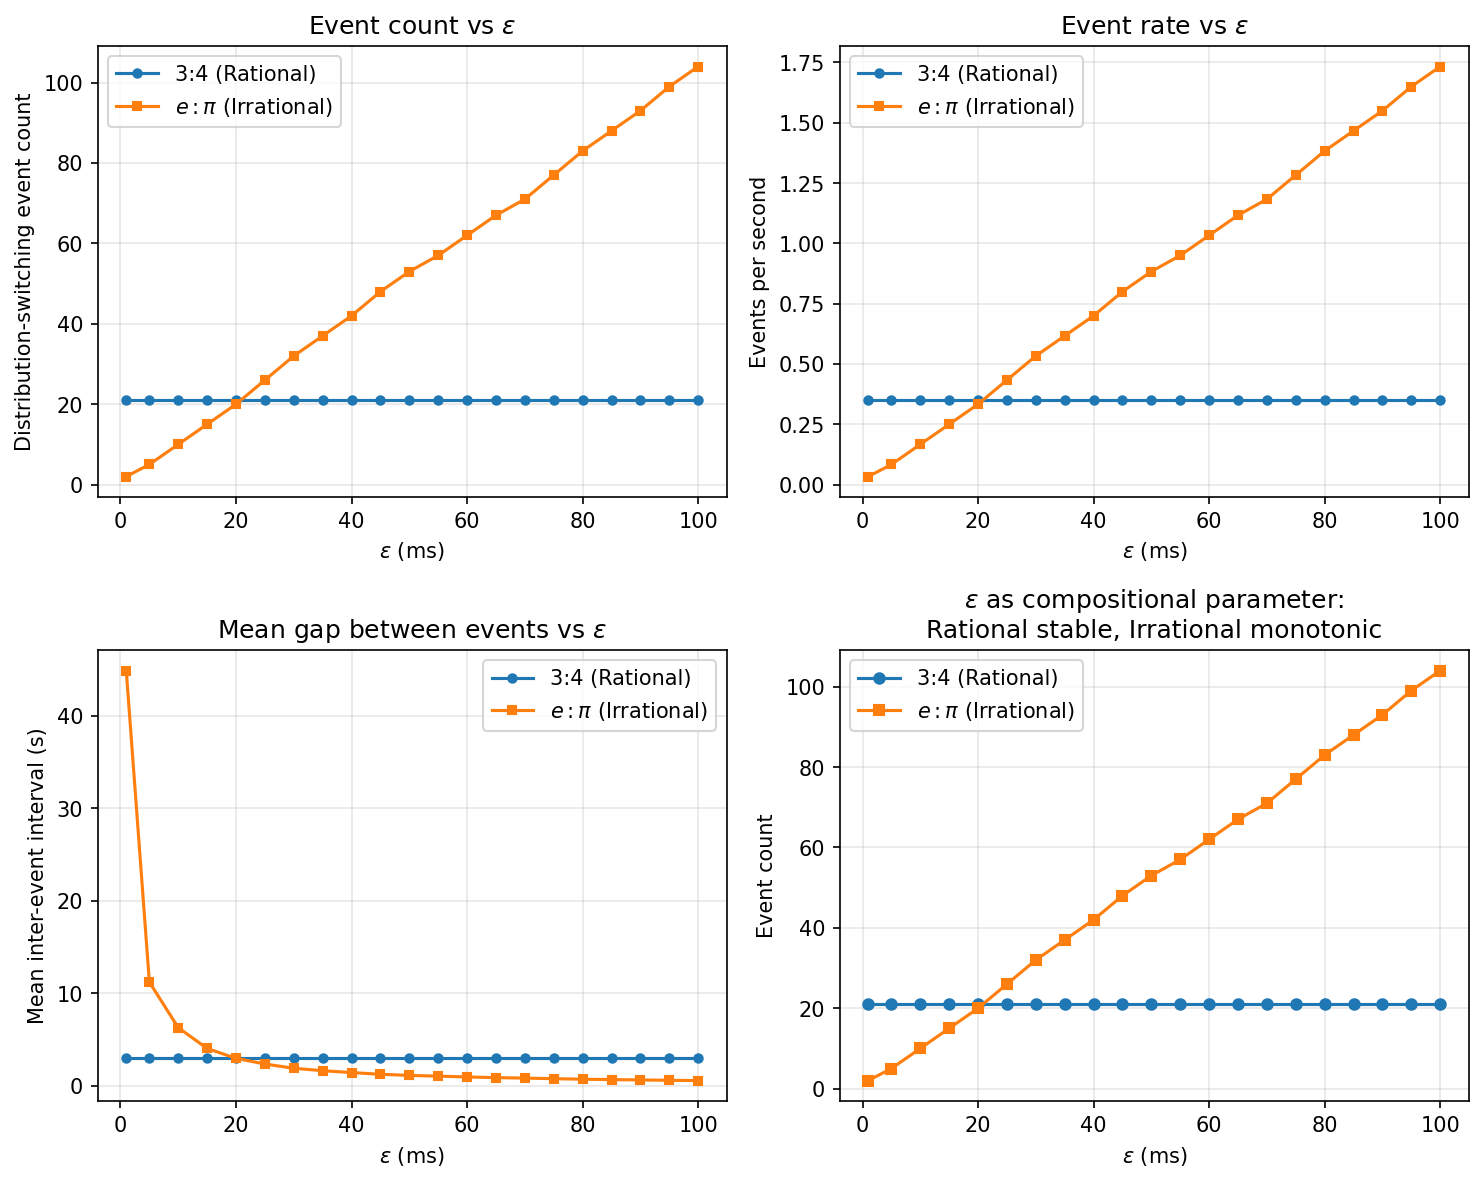
\includegraphics[width=0.95\textwidth]{supplementary_code/experiments/epsilon_sensitivity_cp_full_sweep.png}
\caption{$\epsilon$ sensitivity (full sweep): event count, event rate, and mean inter-event interval over 60~s. Rational 3:4 (blue): count and spacing invariant. Irrational $e:\pi$ (orange): count and rate increase monotonically with $\epsilon$; mean gap decreases. $\epsilon$ thus functions as a compositional parameter for texture transition density.}
\label{fig:epsilon_sensitivity_full}
\end{figure}


\section{nwVSS Weights by Density}
\label{app:nwvss_density}

Applying the same nwVSS weight-extraction procedure (Section~\ref{sec:wvss_validation}) to low-density conditions (20~notes / s aggregate) and high-density (120~notes / s aggregate) yields the weights in Table~\ref{tab:nwvss_density};  The weight shift from high to low density is $-7.81$ percentage points for velocity, $+7.63$ for temporal, and $+0.18$ for pitch. At low density, velocity dominance weakens and temporal (and pitch) components gain relative weight (\emph{weight transfer by density}). The 0.00\% temporal weight at high density is interpretable as computational evidence of temporal fusion: at 120~notes/s, the onset structure ceases to carry discriminative load for separation, which the metric correctly attributes to velocity and pitch.

\begin{table}[htbp]
\tbl{nwVSS weights by aggregate density (same extraction procedure).}
{\begin{tabular}{@{}lrrr@{}} \toprule
Condition & $w_{\text{pitch}}$ (\%) & $w_{\text{vel}}$ (\%) & $w_{\text{temporal}}$ (\%) \\ \midrule
Low density (20~notes/s) & 0.45 & 91.92 & 7.63 \\
High density (120~notes/s) & 0.27 & 99.73 & 0.00 \\ \bottomrule
\end{tabular}}
\tabnote{Weight shift (low minus high): $\Delta w_{\text{pitch}} = +0.18$, $\Delta w_{\text{vel}} = -7.81$, $\Delta w_{\text{temporal}} = +7.63$ percentage points.}
\label{tab:nwvss_density}
\end{table}


\section{Calibration Dataset Audit}
\label{app:audit}

Six publicly available Disklavier-related repositories were audited for velocity-latency calibration data: MAPS Database (audio-MIDI pairs, no velocity sweep), Magenta MIDI Dataset (no hardware-specific latency), MAESTRO (no Disklavier-specific latency characterization), SMD (score-performance alignment only), Vienna 4$\times$22 Piano Corpus (tone quality focus) and RWC Music Database (no systematic latency measurement). \textbf{Finding}: No public dataset pairs MIDI velocity commands with measured acoustic-onset latency for any Disklavier model. Controlled velocity sweeps ($v = 0, 1, \ldots, 1023$; multiple repetitions) with sub-millisecond audio capture are recommended.


\section{Hardware-Aware Actuation Pipeline}
\label{app:algorithm}

Algorithm~\ref{alg:latency} presents the complete adaptive compensation pipeline, which replaces the simplified correction in Algorithm~\ref{alg:generation} (Line~11).

\begin{algorithm}[htbp]
\caption{Hardware-Aware Actuation Pipeline (HAL)}
\label{alg:latency}
\begin{algorithmic}[1]
\Require Event list $E$, calibration data $C$ (optional), compression $\gamma$
\Ensure Compensated event list $E'$
\If{$C$ is available}
    \State $f \gets \textsc{FitPowerLaw}(C)$ \Comment{Best fit: $c \approx 0.5$, RMSE $= 0.69$ ms}
    \State $L(v) \gets 30 - 20 \cdot f(v/1023)$
    \State \textbf{skip} robustness filter
\Else
    \State $L(v) \gets 30 - 20 \cdot (v/1023)$ \Comment{Linear fallback}
\EndIf
\State $E' \gets \emptyset$
\For{each event $(t, p, v, d)$ in $E$}
    \If{$C$ \textbf{not} available \textbf{and} \textsc{IsLatencySensitive}$(E, t, p)$}
        \State $\bar{v} \gets$ mean velocity in $[t-25\text{ms}, t+25\text{ms}]$
        \State $v \gets \bar{v} + \gamma \cdot (v - \bar{v})$ \Comment{$\gamma < 1$: compress}
    \EndIf
    \State $t' \gets t - L(v)/1000$
    \State $E' \gets E' \cup \{(t', p, v, d)\}$
\EndFor
\State \Return $E'$
\end{algorithmic}
\end{algorithm}


\section{Supplementary Materials}
\label{app:supplementary}

Supplementary materials (audio of compositions generated algorithmically by the framework) are available at \url{https://www.amanous.xyz}. These materials document the algorithmically generated output and are for reference and future perceptual experiments; the quantitative results in this paper do not rely on empirical measurement of these recordings. Source code: \url{https://anonymous.4open.science/r/Amanous-2BBF/}.

\textbf{Supplementary excerpts.} The following excerpts are referenced in the text and match the materials on the project website:
\begin{itemize}
    \item \textbf{Excerpt 1:} Demonstration of Beyond-human density rendered in Disklavier (34~s). Polyphony (40-note chords), 30~Hz multi-key trill, 6-octave arpeggio.
    \item \textbf{Excerpt 2:} Phase Music -- Minimalist Study (80~s). Reich-inspired phase-shift; pentatonic set, 1:1.01 tempo drift.
    \item \textbf{Excerpt 3:} Canonical ABAABABA validation composition (74~s). macro-form of the L-system with deterministic sections ($A$) and textural sections ($B$); 3:4 tempo canon.
    \item \textbf{Excerpt 4:} Convergence Point demonstration, 3:4 canon (30~s). Pre-CP sparse/melodic and post-CP dense/ texture switch at $t = 15$~s.
\end{itemize}

Additional materials: (1)~complete MIDI files for all reported experiments; (2)~ablation experiment scripts with deterministic seeds and JSON/CSV output; (3)~analysis reproduction notebooks.

\end{document}